\documentclass[10pt,fleqn]{article} % Default font size and left-justified equations
\usepackage[%
    pdftitle={Modélisation systèmes multiphysiques : Modélisation linéaire et non linéaire},
    pdfauthor={Xavier Pessoles}]{hyperref}
    
%%%%%%%%%%%%%%%%%%%%%%%%%%%%%%%%%%%%%%%%%
% Original author:
% Mathias Legrand (legrand.mathias@gmail.com) with modifications by:
% Vel (vel@latextemplates.com)
% License:
% CC BY-NC-SA 3.0 (http://creativecommons.org/licenses/by-nc-sa/3.0/)
%%%%%%%%%%%%%%%%%%%%%%%%%%%%%%%%%%%%%%%%%

%----------------------------------------------------------------------------------------
%	VARIOUS REQUIRED PACKAGES AND CONFIGURATIONS
%----------------------------------------------------------------------------------------

\usepackage[top=2.5cm,bottom=2cm,left=2cm,right=2cm,headsep=40pt,a4paper]{geometry} % Page margins

\usepackage{graphicx} % Required for including pictures
\graphicspath{{images/}} % Specifies the directory where pictures are stored

\usepackage{lipsum} % Inserts dummy text

\usepackage{tikz} % Required for drawing custom shapes

\usepackage[french]{babel} % English language/hyphenation
\frenchbsetup{StandardLists=true} % Pour éviter la collision babel enumitem pour les listes

\usepackage{enumitem} % Customize lists
\setlist{nolistsep} % Reduce spacing between bullet points and numbered lists

\usepackage{booktabs} % Required for nicer horizontal rules in tables

\usepackage{xcolor} % Required for specifying colors by name
%\definecolor{ocre}{RGB}{243,102,25} % Define the orange color used for highlighting throughout the book
 \definecolor{ocre}{RGB}{49,133,156} % Couleur ''bleue''
\definecolor{violetf}{RGB}{112,48,160} % Couleur ''violet''
\usepackage{enumitem}
\usepackage{pifont} % Pour les dinglist
\usepackage{multicol}
\usepackage{array} % Centrage vertical dans les tableaux

%----------------------------------------------------------------------------------------
%	FONTS
%----------------------------------------------------------------------------------------

\usepackage{avant} % Use the Avantgarde font for headings
%\usepackage{times} % Use the Times font for headings
%\usepackage{mathptmx} % Use the Adobe Times Roman as the default text font together with math symbols from the Sym­bol, Chancery and Com­puter Modern fonts
\usepackage[adobe-utopia]{mathdesign}
\usepackage{microtype} % Slightly tweak font spacing for aesthetics
\usepackage[utf8]{inputenc} % Required for including letters with accents
\usepackage[T1]{fontenc} % Use 8-bit encoding that has 256 glyphs

%----------------------------------------------------------------------------------------
%	BIBLIOGRAPHY AND INDEX
%----------------------------------------------------------------------------------------

\usepackage[style=alphabetic,citestyle=numeric,sorting=nyt,sortcites=true,autopunct=true,babel=hyphen,hyperref=true,abbreviate=false,backref=true,backend=biber]{biblatex}
\addbibresource{bibliography.bib} % BibTeX bibliography file
\defbibheading{bibempty}{}

\usepackage{calc} % For simpler calculation - used for spacing the index letter headings correctly
\usepackage{makeidx} % Required to make an index
\makeindex % Tells LaTeX to create the files required for indexing

%----------------------------------------------------------------------------------------
%	MAIN TABLE OF CONTENTS
%----------------------------------------------------------------------------------------

\usepackage{titletoc} % Required for manipulating the table of contents

\setcounter{tocdepth}{2}     % Dans la table des matieres
\setcounter{secnumdepth}{2}

\contentsmargin{0cm} % Removes the default margin

% Part text styling
\titlecontents{part}[0cm]
{\addvspace{20pt}\centering\large\bfseries}
{}
{}
{}

% Chapter text styling
\titlecontents{chapter}[1.25cm] % Indentation
{\addvspace{12pt}\large\sffamily\bfseries} % Spacing and font options for chapters
{\color{ocre!60}\contentslabel[\Large\thecontentslabel]{1.25cm}\color{ocre}} % Chapter number
{\color{ocre}}  
{\color{ocre!60}\normalsize\;\titlerule*[.5pc]{.}\;\thecontentspage} % Page number

% Section text styling
\titlecontents{section}[1.25cm] % Indentation
{\addvspace{3pt}\sffamily\bfseries} % Spacing and font options for sections
{\color{ocre!60}\contentslabel[\thecontentslabel]{1.25cm} \color{ocre}} % Section number
{\color{ocre}}
{\hfill\color{ocre!60}\thecontentspage} % Page number
[]

% Subsection text styling
\titlecontents{subsection}[1.25cm] % Indentation
{\addvspace{1pt}\sffamily\small} % Spacing and font options for subsections
{\contentslabel[\thecontentslabel]{1.25cm}} % Subsection number
{}
{\ \titlerule*[.5pc]{.}\;\thecontentspage} % Page number
[]


% Subsection text styling
\titlecontents{subsubsection}[1.25cm] % Indentation
{\addvspace{1pt}\sffamily\small} % Spacing and font options for subsections
{\contentslabel[\thecontentslabel]{1.25cm}} % Subsection number
{}
{\ \titlerule*[.5pc]{.}\;\thecontentspage} % Page number
[]

% List of figures
\titlecontents{figure}[0em]
{\addvspace{-5pt}\sffamily}
{\thecontentslabel\hspace*{1em}}
{}
{\ \titlerule*[.5pc]{.}\;\thecontentspage}
[]

% List of tables
\titlecontents{table}[0em]
{\addvspace{-5pt}\sffamily}
{\thecontentslabel\hspace*{1em}}
{}
{\ \titlerule*[.5pc]{.}\;\thecontentspage}
[]

%----------------------------------------------------------------------------------------
%	MINI TABLE OF CONTENTS IN PART HEADS
%----------------------------------------------------------------------------------------

% Chapter text styling
\titlecontents{lchapter}[0em] % Indenting
{\addvspace{15pt}\large\sffamily\bfseries} % Spacing and font options for chapters
{\color{ocre}\contentslabel[\Large\thecontentslabel]{1.25cm}\color{ocre}} % Chapter number
{}  
{\color{ocre}\normalsize\sffamily\bfseries\;\titlerule*[.5pc]{.}\;\thecontentspage} % Page number

% Section text styling
\titlecontents{lsection}[0em] % Indenting
{\sffamily\small} % Spacing and font options for sections
{\contentslabel[\thecontentslabel]{1.25cm}} % Section number
{}
{}

% Subsection text styling
\titlecontents{lsubsection}[.5em] % Indentation
{\normalfont\footnotesize\sffamily} % Font settings
{}
{}
{}

%----------------------------------------------------------------------------------------
%	PAGE HEADERS
%----------------------------------------------------------------------------------------

\usepackage{fancyhdr} % Required for header and footer configuration



\pagestyle{fancy}
 \renewcommand{\headrulewidth}{0pt}
 \fancyhead{}
 \fancyhead[L]{%
 \noindent\begin{minipage}[c]{2.6cm}%
 
\includegraphics[width=2cm]{png/logo_upsti.png}%
 \end{minipage}}

\fancyhead[C]{\rule{8cm}{.5pt}}

 \fancyhead[R]{%
 \noindent\begin{minipage}[c]{3cm}
 \begin{flushright}
 \footnotesize{\textit{\textsf{\xxtete}}}%
 \end{flushright}
 \end{minipage}
}


\fancyfoot[C]{\rule{12cm}{.5pt}}
\renewcommand{\footrulewidth}{0.2pt}
\fancyfoot[C]{\footnotesize{\bfseries \thepage}}
\fancyfoot[L]{ 
\begin{minipage}[c]{.4\linewidth}
\noindent\footnotesize{{\xxauteur}}
\end{minipage}}


\fancyfoot[R]{\footnotesize{\xxpied}
\ifthenelse{\isodd{\value{page}}}{
\begin{tikzpicture}[overlay]
\node[shape=rectangle, 
      rounded corners = .25 cm,
	  draw= ocre,
	  line width=2pt, 
	  fill = ocre!10,
	  minimum width  = 2.5cm,
	  minimum height = 3cm,] at (\xxposongletx,\xxposonglety) {};
\node at (\xxposonglettext,\xxposonglety) {\rotatebox{90}{\textbf{\large\color{ocre}{\xxonglet}}}};
%{};
\end{tikzpicture}}{}
}
%
%
%
% Removes the header from odd empty pages at the end of chapters
\makeatletter
\renewcommand{\cleardoublepage}{
\clearpage\ifodd\c@page\else
\hbox{}
\vspace*{\fill}
\thispagestyle{empty}
\newpage
\fi}

\fancypagestyle{plain}{%
\fancyhf{} % vide l’en-tête et le pied~de~page.
%\fancyfoot[C]{\bfseries \thepage} % numéro de la page en cours en gras
% et centré en pied~de~page.
\fancyfoot[R]{\footnotesize{\xxpied}}
\fancyfoot[C]{\rule{12cm}{.5pt}}
\renewcommand{\footrulewidth}{0.2pt}
\fancyfoot[C]{\footnotesize{\bfseries \thepage}}
\fancyfoot[L]{ 
\begin{minipage}[c]{.4\linewidth}
\noindent\footnotesize{{\xxauteur}}
\end{minipage}}}



%----------------------------------------------------------------------------------------
%	THEOREM STYLES
%----------------------------------------------------------------------------------------

% Conflit avec la police adobe
%\usepackage{amsmath,amsfonts,amssymb,amsthm} % For math equations, theorems, symbols, etc
\usepackage{amsmath,amsthm}

\newcommand{\intoo}[2]{\mathopen{]}#1\,;#2\mathclose{[}}
\newcommand{\ud}{\mathop{\mathrm{{}d}}\mathopen{}}
\newcommand{\intff}[2]{\mathopen{[}#1\,;#2\mathclose{]}}
%\newtheorem{notation}{Notation}[chapter]
\newtheorem{notation}{Notation}[section]

% Boxed/framed environments
\newtheoremstyle{ocrenumbox}% % Theorem style name
{0pt}% Space above
{0pt}% Space below
{\normalfont}% % Body font
{}% Indent amount
{\small\bf\sffamily\color{ocre}}% % Theorem head font
{\;}% Punctuation after theorem head
{0.25em}% Space after theorem head
{\small\sffamily\color{ocre}\thmname{#1}\nobreakspace\thmnumber%{\@ifnotempty{#1}{}\@upn{#2}}% Theorem text (e.g. Theorem 2.1)
\thmnote{\nobreakspace\the\thm@notefont\sffamily\bfseries\color{black}---\nobreakspace#3.}} % Optional theorem note
\renewcommand{\qedsymbol}{$\blacksquare$}% Optional qed square


% Boite pour les corriges
\newtheoremstyle{correctionbox}% % Theorem style name
{0pt}% Space above
{0pt}% Space below
{\normalfont}% % Body font
{}% Indent amount
{\small\bf\sffamily\color{violet}}% % Theorem head font
{\;}% Punctuation after theorem head
{0.25em}% Space after theorem head
{\small\sffamily\color{ocre}\thmname{#1}\nobreakspace\thmnumber%{\@ifnotempty{#1}{}\@upn{#2}}% Theorem text (e.g. Theorem 2.1)
\thmnote{\nobreakspace\the\thm@notefont\sffamily\bfseries\color{black}---\nobreakspace#3.}} % Optional theorem note
\renewcommand{\qedsymbol}{$\blacksquare$}% Optional qed square



\newtheoremstyle{blacknumex}% Theorem style name
{5pt}% Space above
{5pt}% Space below
{\normalfont}% Body font
{} % Indent amount
{\small\bf\sffamily}% Theorem head font
{\;}% Punctuation after theorem head
{0.25em}% Space after theorem head
{\small\sffamily{\tiny\ensuremath{\blacksquare}}\nobreakspace\thmname{#1}\nobreakspace\thmnumber%{\@ifnotempty{#1}{}\@upn{#2}}% Theorem text (e.g. Theorem 2.1)
\thmnote{\nobreakspace\the\thm@notefont\sffamily\bfseries---\nobreakspace#3.}}% Optional theorem note

\newtheoremstyle{blacknumbox} % Theorem style name
{0pt}% Space above
{0pt}% Space below
{\normalfont}% Body font
{}% Indent amount
{\small\bf\sffamily}% Theorem head font
{\;}% Punctuation after theorem head
{0.25em}% Space after theorem head
{\small\sffamily\thmname{#1}\nobreakspace 
\thmnote{\nobreakspace\the\thm@notefont\sffamily\bfseries---\nobreakspace#3.}}% Optional theorem note

% Non-boxed/non-framed environments
\newtheoremstyle{ocrenum}% % Theorem style name
{5pt}% Space above
{5pt}% Space below
{\normalfont}% % Body font
{}% Indent amount
{\small\bf\sffamily\color{ocre}}% % Theorem head font
{\;}% Punctuation after theorem head
{0.25em}% Space after theorem head
{\small\sffamily\color{ocre}\thmname{#1}\nobreakspace%\thmnumber{\@ifnotempty{#1}{}\@upn{#2}}% Theorem text (e.g. Theorem 2.1)
\thmnote{\nobreakspace\the\thm@notefont\sffamily\bfseries\color{black}---\nobreakspace#3.}} % Optional theorem note
\renewcommand{\qedsymbol}{$\blacksquare$}% Optional qed square
\makeatother

% Environnement pour les titres de parties
\newtheoremstyle{partiebox} 
{0pt}% Space above
{0pt}% Space below
{\normalfont}% Body font
{}% Indent amount
{\small\bf\sffamily}% Theorem head font
{\;}% Punctuation after theorem head
{0.25em}% Space after theorem head




% Defines the theorem text style for each type of theorem to one of the three styles above
\newcounter{dummy} 
\numberwithin{dummy}{section}
\theoremstyle{ocrenumbox}
%\newtheorem{theoremeT}[dummy]{Théorème}
\newtheorem{theoremeT}[dummy]{Théorème}
\newtheorem{resultatT}[dummy]{Résultat}
\newtheorem{savoirT}[dummy]{Savoir}
\newtheorem{methodeT}[dummy]{Méthode}
\newtheorem{objectifT}[dummy]{Objectif}
%\newtheorem{problem}{Problem}[chapter]
\newtheorem{problem}{Problem}[section]
%\newtheorem{exerciseT}{Exercise}[chapter]
\newtheorem{exerciseT}{Exercice}[section]

\theoremstyle{blacknumex}
%\newtheorem{exampleT}{Example}[chapter]
\newtheorem{exempleT}{Exemple}[section]
\newtheorem{termT}{Terminal\\}[section]
\newtheorem{pyT}{Python\\}[section]
\newtheorem{sciT}{Scilab\\}[section]
\newtheorem{pseudoT}{Pseudo Code\\}[section]
\newtheorem{sqlT}{SQL\\}[section]

\theoremstyle{blacknumbox}
%\newtheorem{vocabulary}{Vocabulary}[chapter]
\newtheorem{vocabulary}{Vocabulaire}[section]
%\newtheorem{definitionT}{Definition}[section]
\newtheorem{definitionT}{Définition}[section]
\newtheorem{rappelT}{Rappel}[section]
\newtheorem{demoT}{Démonstration}[section]
\newtheorem{corollaryT}[dummy]{Corollaire}
\newtheorem{hypoT}{Hypothèse(s)}

\theoremstyle{ocrenum}
\newtheorem{proposition}[dummy]{Proposition}

\theoremstyle{partiebox}
\newtheorem{titrepartieT}[]{}
\newtheorem{titrechapitreT}[]{}

\theoremstyle{correctionbox}
\newtheorem{correctionT}[dummy]{\color{violet}{Correction}}

%----------------------------------------------------------------------------------------
%	DEFINITION OF COLORED BOXES
%----------------------------------------------------------------------------------------

\RequirePackage[framemethod=tikz]{mdframed} % Required for creating the theorem, definition, exercise and corollary boxes

% Theorem box
\newmdenv[skipabove=7pt,
skipbelow=7pt,
backgroundcolor=ocre!10,
linecolor=ocre,
innerleftmargin=5pt,
innerrightmargin=5pt,
innertopmargin=5pt,
leftmargin=0cm,
rightmargin=0cm,
innerbottommargin=5pt]{tBox}


% Correction
\newmdenv[skipabove=7pt,
skipbelow=7pt,
backgroundcolor=violet!10,
linecolor=violet,
innerleftmargin=5pt,
innerrightmargin=5pt,
innertopmargin=5pt,
leftmargin=0cm,
rightmargin=0cm,
innerbottommargin=5pt]{coBox}


% Exercise box	  
\newmdenv[skipabove=7pt,
skipbelow=7pt,
rightline=false,
leftline=true,
topline=false,
bottomline=false,
backgroundcolor=ocre!10,
linecolor=ocre,
innerleftmargin=5pt,
innerrightmargin=5pt,
innertopmargin=5pt,
innerbottommargin=5pt,
leftmargin=0cm,
rightmargin=0cm,
linewidth=4pt]{eBox}	

% Definition box
\newmdenv[skipabove=7pt,
skipbelow=7pt,
rightline=false,
leftline=true,
topline=false,
bottomline=false,
backgroundcolor=ocre!10,
linecolor=ocre,
innerleftmargin=5pt,
innerrightmargin=5pt,
innertopmargin=0pt,
leftmargin=0cm,
rightmargin=0cm,
linewidth=4pt,
innerbottommargin=0pt]{dBox}	

% Demonstration box
\newmdenv[skipabove=7pt,
skipbelow=7pt,
rightline=false,
leftline=true,
topline=false,
bottomline=false,
%backgroundcolor=ocre!10,
linecolor=ocre,
innerleftmargin=5pt,
innerrightmargin=5pt,
innertopmargin=0pt,
leftmargin=0cm,
rightmargin=0cm,
linewidth=4pt,
innerbottommargin=0pt]{demoBox}	

% Corollary box
\newmdenv[skipabove=7pt,
skipbelow=7pt,
rightline=false,
leftline=true,
topline=false,
bottomline=false,
linecolor=gray,
backgroundcolor=black!5,
innerleftmargin=5pt,
innerrightmargin=5pt,
innertopmargin=5pt,
leftmargin=0cm,
rightmargin=0cm,
linewidth=4pt,
innerbottommargin=5pt]{cBox}


% Hypothèses
\newmdenv[skipabove=7pt,
skipbelow=7pt,
rightline=false,
leftline=true,
topline=false,
bottomline=false,
linecolor=gray,
backgroundcolor=black!5,
innerleftmargin=5pt,
innerrightmargin=5pt,
innertopmargin=5pt,
leftmargin=0cm,
rightmargin=0cm,
linewidth=4pt,
innerbottommargin=5pt]{hyBox}


% Boite pour le titre de la partie (pBox)
\newmdenv[skipabove=7pt,
skipbelow=7pt,
rightline=true,
leftline=false,
topline=false,
bottomline=false,
linecolor=ocre,
backgroundcolor=none,
innerleftmargin=5pt,
innerrightmargin=5pt,
innertopmargin=5pt,
leftmargin=0cm,
rightmargin=0cm,
linewidth=4pt,
innerbottommargin=5pt]{pBox}

% Boite pour le titre du chapitre (chBox)
\newmdenv[skipabove=7pt,
skipbelow=7pt,
rightline=false,
leftline=true,
topline=false,
bottomline=false,
linecolor=ocre,
%backgroundcolor=black!5,
innerleftmargin=5pt,
innerrightmargin=5pt,
innertopmargin=5pt,
leftmargin=0cm,
rightmargin=0cm,
linewidth=4pt,
innerbottommargin=5pt]{chBox}


% Boite pour les exemples
\newmdenv[skipabove=7pt,
skipbelow=7pt,
rightline=false,
leftline=true,
topline=false,
bottomline=false,
linecolor=gray,
backgroundcolor=white,
innerleftmargin=5pt,
innerrightmargin=5pt,
innertopmargin=5pt,
leftmargin=0cm,
rightmargin=0cm,
linewidth=4pt,
innerbottommargin=5pt]{exBox}

% Boite pour le terminal
\newmdenv[skipabove=7pt,
skipbelow=7pt,
rightline=false,
leftline=true,
topline=false,
bottomline=false,
linecolor=gray,
backgroundcolor=white,
innerleftmargin=5pt,
innerrightmargin=5pt,
innertopmargin=5pt,
leftmargin=0cm,
rightmargin=0cm,
linewidth=4pt,
innerbottommargin=5pt]{termBox}


% Boite pour Python
\newmdenv[skipabove=7pt,
skipbelow=7pt,
rightline=false,
leftline=true,
topline=false,
bottomline=false,
linecolor=gray,
backgroundcolor=white,
innerleftmargin=5pt,
innerrightmargin=5pt,
innertopmargin=0pt,
leftmargin=0cm,
rightmargin=0cm,
linewidth=4pt,
innerbottommargin=5pt]{pyBox}

% Boite pour scilab
\newmdenv[skipabove=7pt,
skipbelow=7pt,
rightline=false,
leftline=true,
topline=false,
bottomline=false,
linecolor=gray,
backgroundcolor=white,
innerleftmargin=5pt,
innerrightmargin=5pt,
innertopmargin=5pt,
leftmargin=0cm,
rightmargin=0cm,
linewidth=4pt,
innerbottommargin=5pt]{sciBox}


% Boite pour pseudo
\newmdenv[skipabove=7pt,
skipbelow=7pt,
rightline=false,
leftline=true,
topline=false,
bottomline=false,
linecolor=gray,
backgroundcolor=white,
innerleftmargin=5pt,
innerrightmargin=5pt,
innertopmargin=5pt,
leftmargin=0cm,
rightmargin=0cm,
linewidth=4pt,
innerbottommargin=5pt]{pseudoBox}

% Boite pour pseudo
\newmdenv[skipabove=7pt,
skipbelow=7pt,
rightline=false,
leftline=true,
topline=false,
bottomline=false,
linecolor=gray,
backgroundcolor=white,
innerleftmargin=5pt,
innerrightmargin=5pt,
innertopmargin=5pt,
leftmargin=0cm,
rightmargin=0cm,
linewidth=4pt,
innerbottommargin=5pt]{sqlBox}


% Creates an environment for each type of theorem and assigns it a theorem text style from the "Theorem Styles" section above and a colored box from above
\newenvironment{theorem}{\begin{tBox}\begin{theoremeT}}{\end{theoremeT}\end{tBox}}
\newenvironment{resultat}{\begin{tBox}\begin{resultatT}}{\end{resultatT}\end{tBox}}
\newenvironment{methode}{\begin{tBox}\begin{methodeT}}{\end{methodeT}\end{tBox}}
\newenvironment{savoir}{\begin{tBox}\begin{savoirT}}{\end{savoirT}\end{tBox}}
\newenvironment{obj}{\begin{tBox}\begin{objectifT}}{\end{objectifT}\end{tBox}}
\newenvironment{corrige}{\begin{coBox}\begin{correctionT}}{\end{correctionT}\end{coBox}}
\newenvironment{exercise}{\begin{eBox}\begin{exerciseT}}{\hfill{\color{ocre}\tiny\ensuremath{\blacksquare}}\end{exerciseT}\end{eBox}}				  
\newenvironment{exercice}{\begin{eBox}\begin{exerciseT}}{\hfill{\color{ocre}\tiny\ensuremath{\blacksquare}}\end{exerciseT}\end{eBox}}				  

\newenvironment{definition}{\begin{dBox}\begin{definitionT}}{\end{definitionT}\end{dBox}}	
\newenvironment{rappel}{\begin{dBox}\begin{rappelT}}{\end{rappelT}\end{dBox}}	
\newenvironment{defi}{\begin{dBox}\begin{definitionT}}{\end{definitionT}\end{dBox}}	
\newenvironment{demo}{\begin{demoBox}\begin{demoT}}{\end{demoT}\end{demoBox}}	
%\newenvironment{exemple}{\begin{exempleT}}{\hfill{\tiny\ensuremath{\blacksquare}}\end{exempleT}}		
\newenvironment{corollary}{\begin{cBox}\begin{corollaryT}}{\end{corollaryT}\end{cBox}}
\newenvironment{hypo}{\begin{hyBox}\begin{hypoT}}{\end{hypoT}\end{hyBox}}	\newenvironment{exemple}{\begin{exBox}\begin{exempleT}}{\hfill{\tiny\ensuremath{\blacksquare}}\end{exempleT}\end{exBox}}	
\newenvironment{titrepartie}{\begin{pBox}\begin{titrepartieT}}{\end{titrepartieT}\end{pBox}}	
\newenvironment{titrechapitre}{\begin{chBox}\begin{titrechapitreT}}{\end{titrechapitreT}\end{chBox}}	

\newenvironment{term}{ \begin{termBox}\begin{termT}}{\end{termT}\end{termBox}}
\newenvironment{py}{ \begin{pyBox}\begin{pyT}}{\end{pyT}\end{pyBox}}
\newenvironment{sci}{ \begin{sciBox}\begin{sciT}}{\end{sciT}\end{sciBox}}
\newenvironment{pseudo}{ \begin{pseudoBox}\begin{pseudoT}}{\end{pseudoT}\end{pseudoBox}}
\newenvironment{envsql}{ \begin{sqlBox}\begin{sqlT}}{\end{sqlT}\end{sqlBox}}


%----------------------------------------------------------------------------------------
%	REMARK ENVIRONMENT
%----------------------------------------------------------------------------------------

\newenvironment{remark}{\par\vspace{10pt}\small % Vertical white space above the remark and smaller font size
\begin{list}{}{
\leftmargin=35pt % Indentation on the left
\rightmargin=25pt}\item\ignorespaces % Indentation on the right
\makebox[-2.5pt]{\begin{tikzpicture}[overlay]
\node[draw=ocre!60,line width=1pt,circle,fill=ocre!25,font=\sffamily\bfseries,inner sep=2pt,outer sep=0pt] at (-15pt,0pt){\textcolor{ocre}{R}};\end{tikzpicture}} % Orange R in a circle
\advance\baselineskip -1pt}{\end{list}\vskip5pt} % Tighter line spacing and white space after remark

\newenvironment{rem}{\par\vspace{10pt}\small % Vertical white space above the remark and smaller font size
\begin{list}{}{
\leftmargin=35pt % Indentation on the left
\rightmargin=25pt}\item\ignorespaces % Indentation on the right
\makebox[-2.5pt]{\begin{tikzpicture}[overlay]
\node[draw=ocre!60,line width=1pt,circle,fill=ocre!25,font=\sffamily\bfseries,inner sep=2pt,outer sep=0pt] at (-15pt,0pt){\textcolor{ocre}{R}};\end{tikzpicture}} % Orange R in a circle
\advance\baselineskip -1pt}{\end{list}\vskip5pt} % Tighter line spacing and white space after remark


\newenvironment{warn}{\par\vspace{10pt}\small % Vertical white space above the remark and smaller font size
\begin{list}{}{
\leftmargin=35pt % Indentation on the left
\rightmargin=25pt}\item\ignorespaces % Indentation on the right
\makebox[-2.5pt]{\begin{tikzpicture}[overlay]
\node[draw=red!60,line width=1pt,circle,fill=red!25,font=\sffamily\bfseries,inner sep=2pt,outer sep=0pt] at (-15pt,0pt){\textcolor{black}{!}};\end{tikzpicture}} % Point d'exclamation dans un cercle
\advance\baselineskip -1pt}{\end{list}\vskip5pt} % Tighter line spacing and white space after remark


%----------------------------------------------------------------------------------------
%	SECTION NUMBERING IN THE MARGIN
%----------------------------------------------------------------------------------------
\setcounter{secnumdepth}{3}
\setcounter{tocdepth}{2}



\makeatletter
\renewcommand{\@seccntformat}[1]{\llap{\textcolor{ocre}{\csname the#1\endcsname}\hspace{1em}}}                    
\renewcommand{\section}{\@startsection{section}{1}{\z@}
{-4ex \@plus -1ex \@minus -.4ex}
{1ex \@plus.2ex }
{\normalfont\large\sffamily\bfseries}}
\renewcommand{\subsection}{\@startsection {subsection}{2}{\z@}
{-3ex \@plus -0.1ex \@minus -.4ex}
{0.5ex \@plus.2ex }
{\normalfont\sffamily\bfseries}}
\renewcommand{\subsubsection}{\@startsection {subsubsection}{3}{\z@}
{-2ex \@plus -0.1ex \@minus -.2ex}
{.2ex \@plus.2ex }
{\normalfont\small\sffamily\bfseries}}                        
\renewcommand\paragraph{\@startsection{paragraph}{4}{\z@}
{-2ex \@plus-.2ex \@minus .2ex}
{.1ex}
{\normalfont\small\sffamily\bfseries}}

%----------------------------------------------------------------------------------------
%	PART HEADINGS
%----------------------------------------------------------------------------------------


%----------------------------------------------------------------------------------------
%	CHAPTER HEADINGS
%----------------------------------------------------------------------------------------

% \newcommand{\thechapterimage}{}%
% \newcommand{\chapterimage}[1]{\renewcommand{\thechapterimage}{#1}}%
% \def\@makechapterhead#1{%
% {\parindent \z@ \raggedright \normalfont
% \ifnum \c@secnumdepth >\m@ne
% \if@mainmatter
% \begin{tikzpicture}[remember picture,overlay]
% \node at (current page.north west)
% {\begin{tikzpicture}[remember picture,overlay]
% \node[anchor=north west,inner sep=0pt] at (0,0) {\includegraphics[width=\paperwidth]{\thechapterimage}};
% \draw[anchor=west] (\Gm@lmargin,-9cm) node [line width=2pt,rounded corners=15pt,draw=ocre,fill=white,fill opacity=0.5,inner sep=15pt]{\strut\makebox[22cm]{}};
% \draw[anchor=west] (\Gm@lmargin+.3cm,-9cm) node {\huge\sffamily\bfseries\color{black}\thechapter. #1\strut};
% \end{tikzpicture}};
% \end{tikzpicture}
% \else
% \begin{tikzpicture}[remember picture,overlay]
% \node at (current page.north west)
% {\begin{tikzpicture}[remember picture,overlay]
% \node[anchor=north west,inner sep=0pt] at (0,0) {\includegraphics[width=\paperwidth]{\thechapterimage}};
% \draw[anchor=west] (\Gm@lmargin,-9cm) node [line width=2pt,rounded corners=15pt,draw=ocre,fill=white,fill opacity=0.5,inner sep=15pt]{\strut\makebox[22cm]{}};
% \draw[anchor=west] (\Gm@lmargin+.3cm,-9cm) node {\huge\sffamily\bfseries\color{black}#1\strut};
% \end{tikzpicture}};
% \end{tikzpicture}
% \fi\fi\par\vspace*{270\p@}}}

%-------------------------------------------

\def\@makeschapterhead#1{%
\begin{tikzpicture}[remember picture,overlay]
\node at (current page.north west)
{\begin{tikzpicture}[remember picture,overlay]
\node[anchor=north west,inner sep=0pt] at (0,0) {\includegraphics[width=\paperwidth]{\thechapterimage}};
\draw[anchor=west] (\Gm@lmargin,-9cm) node [line width=2pt,rounded corners=15pt,draw=ocre,fill=white,fill opacity=0.5,inner sep=15pt]{\strut\makebox[22cm]{}};
\draw[anchor=west] (\Gm@lmargin+.3cm,-9cm) node {\huge\sffamily\bfseries\color{black}#1\strut};
\end{tikzpicture}};
\end{tikzpicture}
\par\vspace*{270\p@}}
\makeatother

%----------------------------------------------------------------------------------------
%	HYPERLINKS IN THE DOCUMENTS
%----------------------------------------------------------------------------------------


\hypersetup{hidelinks,backref=true,pagebackref=true,hyperindex=true,colorlinks=false,breaklinks=true,urlcolor= ocre,bookmarks=true,bookmarksopen=false,pdftitle={Title},pdfauthor={Author}}
\usepackage{bookmark}
\bookmarksetup{
open,
numbered,
addtohook={%
\ifnum\bookmarkget{level}=0 % chapter
\bookmarksetup{bold}%
\fi
\ifnum\bookmarkget{level}=-1 % part
\bookmarksetup{color=ocre,bold}%
\fi
}
}

%----------------------------------------------------------------------------------------
%	
%----------------------------------------------------------------------------------------

\newcommand{\thechapterimage}{}%
\newcommand{\chapterimage}[1]{\renewcommand{\thechapterimage}{#1}}%
\def\@makechapterhead#1{%
{\parindent \z@ \raggedright \normalfont
\begin{tikzpicture}[remember picture,overlay]
\node at (current page.north west)
{\begin{tikzpicture}[remember picture,overlay]
\node[anchor=north west,inner sep=0pt] at (0,0) {\includegraphics[width=\paperwidth]{\thechapterimage}};
%\draw[anchor=west] (\Gm@lmargin,-9cm) node [line width=2pt,rounded corners=15pt,draw=ocre,fill=white,fill opacity=0.5,inner sep=15pt]{\strut\makebox[22cm]{}};
%\draw[anchor=west] (\Gm@lmargin+.3cm,-9cm) node {\huge\sffamily\bfseries\color{black}\thechapter. #1\strut};
\end{tikzpicture}};
\end{tikzpicture}
\par\vspace*{270\p@}
}}

 \newcounter{exo}


\makeatletter             
\renewcommand{\subparagraph}{\@startsection{exo}{5}{\z@}%
                                    {-2ex \@plus-.2ex \@minus .2ex}%
                                    {0ex}%               
{\normalfont\bfseries Question \hspace{.7cm} }}
\makeatother
\renewcommand{\thesubparagraph}{\arabic{subparagraph}} 
\makeatletter


%%%% Environnement pour inclure du code
\usepackage{textcomp}
\usepackage[french]{algorithm2e}
\usepackage{listings}
\lstloadlanguages{R}   % pour regler les pb d accent utf8 dans les codes
\lstset{language=R} % pour regler les pb d accent utf8 dans les codes
\renewcommand{\lstlistlistingname}{Listings}
\renewcommand{\lstlistingname}{Listing}

\SetKwBlock{Fonction}{Début Fonction}{Fin Fonction}
\SetKwComment{Comment}{start}{end}

\definecolor{Bleu}{rgb}{0.1,0.1,1.0}
\definecolor{Noir}{rgb}{0,0,0}
\definecolor{Grau}{rgb}{0.5,0.5,0.5}
\definecolor{DunkelGrau}{rgb}{0.15,0.15,0.15}
\definecolor{Hellbraun}{rgb}{0.5,0.25,0.0}
\definecolor{Magenta}{rgb}{1.0,0.0,1.0}
\definecolor{Gris}{gray}{0.5}
\definecolor{Vert}{rgb}{0,0.5,0}
\definecolor{SourceHintergrund}{rgb}{1,1.0,0.95}


\lstnewenvironment{python}[1][]{
\lstset{
%escapeinside={\%*}{*)},
inputencoding=utf8,   % pour regler les pb d accent utf8 dans les codes
extendedchars=true,   % pour regler les pb d accent utf8 dans les codes
language=python,
basicstyle=\ttfamily\footnotesize, 	
stringstyle=\color{red}, 
showstringspaces=false, 
alsoletter={1234567890},
otherkeywords={\ , \}, \{},
keywordstyle=\color{blue},
emph={access,and,break,class,continue,def,del,elif ,else,
except,exec,finally,for,from,global,if,import,in,i s,
lambda,not,or,pass,print,raise,return,try,while},
emphstyle=\color{black}\bfseries,
emph={[2]True, False, None, self},
emphstyle=[2]\color{black},
emph={[3]from, import, as},
emphstyle=[3]\color{blue},
upquote=true,
columns=flexible, % pour empecher d'avoir un espacement mono
morecomment=[s]{"""}{"""},
commentstyle=\color{Hellbraun}\slshape, 
%emph={[4]1, 2, 3, 4, 5, 6, 7, 8, 9, 0},
emphstyle=[4]\color{blue},
literate=*{:}{{\textcolor{blue}:}}{1}
{=}{{\textcolor{blue}=}}{1}
{-}{{\textcolor{blue}-}}{1}
{+}{{\textcolor{blue}+}}{1}
{*}{{\textcolor{blue}*}}{1}
{!}{{\textcolor{blue}!}}{1}
{(}{{\textcolor{blue}(}}{1}
{)}{{\textcolor{blue})}}{1}
{[}{{\textcolor{blue}[}}{1}
{]}{{\textcolor{blue}]}}{1}
{<}{{\textcolor{blue}<}}{1}
{>}{{\textcolor{blue}>}}{1}
{COMPLETER}{{\textcolor{red}COMPLETER}}{1},
literate=%
            {é}{{\'{e}}}1
            {è}{{\`{e}}}1
            {ê}{{\^{e}}}1
            {ë}{{\¨{e}}}1
            {û}{{\^{u}}}1
            {ù}{{\`{u}}}1
            {â}{{\^{a}}}1
            {à}{{\`{a}}}1
            {î}{{\^{i}}}1
            {ç}{{\c{c}}}1
            {Ç}{{\c{C}}}1
            {É}{{\'{E}}}1
            {Ê}{{\^{E}}}1
            {À}{{\`{A}}}1
            {Â}{{\^{A}}}1
            {Î}{{\^{I}}}1, % pour regler les pb d accent utf8 dans les codes
%framexleftmargin=1mm, framextopmargin=1mm, frame=shadowbox, rulesepcolor=\color{blue},#1
%backgroundcolor=\color{SourceHintergrund}, 
%framexleftmargin=1mm, framexrightmargin=1mm, framextopmargin=1mm, frame=single, framerule=1pt, rulecolor=\color{black},#1
}}{}



\lstnewenvironment{scilab}[1][]{
\lstset{
language=scilab,
basicstyle=\sffamily\footnotesize, 	
stringstyle=\color{red}, 
showstringspaces=false, 
alsoletter={1234567890},
otherkeywords={\ , \}, \{},
keywordstyle=\color{blue},
emph={access,and,break,class,continue,def,del,elif ,else,
except,exec,finally,for,from,global,if,import,in,i s,
lambda,not,or,pass,print,raise,return,try,while,Debut},
emphstyle=\color{black}\bfseries,
emph={[2]True, False, None, self},
emphstyle=[2]\color{black},
emph={[3]from, import, as},
emphstyle=[3]\color{blue},
upquote=true,
columns=flexible, % pour empecher d'avoir un espacement mono
morecomment=[s]{"""}{"""},
commentstyle=\color{Hellbraun}\slshape, 
%emph={[4]1, 2, 3, 4, 5, 6, 7, 8, 9, 0},
emphstyle=[4]\color{blue},
literate=*{:}{{\textcolor{blue}:}}{1}
{=}{{\textcolor{blue}=}}{1}
{-}{{\textcolor{blue}-}}{1}
{+}{{\textcolor{blue}+}}{1}
{*}{{\textcolor{blue}*}}{1}
{!}{{\textcolor{blue}!}}{1}
{(}{{\textcolor{blue}(}}{1}
{)}{{\textcolor{blue})}}{1}
{[}{{\textcolor{blue}[}}{1}
{]}{{\textcolor{blue}]}}{1}
{<}{{\textcolor{blue}<}}{1}
{>}{{\textcolor{blue}>}}{1},
%framexleftmargin=1mm, framextopmargin=1mm, frame=shadowbox, rulesepcolor=\color{blue},#1
%backgroundcolor=\color{SourceHintergrund}, 
%framexleftmargin=1mm, framexrightmargin=1mm, framextopmargin=1mm, frame=single, framerule=1pt, rulecolor=\color{black},#1
}}{}


\lstdefinestyle{stylepython}{%
escapeinside={\%*}{*)},
inputencoding=utf8,   % pour regler les pb d accent utf8 dans les codes
extendedchars=true,   % pour regler les pb d accent utf8 dans les codes
language=python,
basicstyle=\sffamily\footnotesize, 	
stringstyle=\color{red}, 
showstringspaces=false, 
alsoletter={1234567890},
otherkeywords={\ , \}, \{},
keywordstyle=\color{blue},
emph={access,and,break,class,continue,def,del,elif ,else,
except,exec,finally,for,from,global,if,import,in,i s,
lambda,not,or,pass,print,raise,return,try,while},
emphstyle=\color{black}\bfseries,
emph={[2]True, False, None, self},
emphstyle=[2]\color{green},
emph={[3]from, import, as},
emphstyle=[3]\color{blue},
upquote=true,
columns=flexible, % pour empecher d'avoir un espacement mono
morecomment=[s]{"""}{"""},
commentstyle=\color{Hellbraun}\slshape, 
%emph={[4]1, 2, 3, 4, 5, 6, 7, 8, 9, 0},
emphstyle=[4]\color{blue},
literate=*{:}{{\textcolor{blue}:}}{1}
{=}{{\textcolor{blue}=}}{1}
{-}{{\textcolor{blue}-}}{1}
{+}{{\textcolor{blue}+}}{1}
{*}{{\textcolor{blue}*}}{1}
{!}{{\textcolor{blue}!}}{1}
{(}{{\textcolor{blue}(}}{1}
{)}{{\textcolor{blue})}}{1}
{[}{{\textcolor{blue}[}}{1}
{]}{{\textcolor{blue}]}}{1}
{<}{{\textcolor{blue}<}}{1}
{>}{{\textcolor{blue}>}}{1}
{COMPLETER}{{\textcolor{red}COMPLETER}}{1},
literate=%
            {é}{{\'{e}}}1
            {è}{{\`{e}}}1
            {ê}{{\^{e}}}1
            {ë}{{\¨{e}}}1
            {û}{{\^{u}}}1
            {ù}{{\`{u}}}1
            {â}{{\^{a}}}1
            {à}{{\`{a}}}1
            {î}{{\^{i}}}1
            {ç}{{\c{c}}}1
            {Ç}{{\c{C}}}1
            {É}{{\'{E}}}1
            {Ê}{{\^{E}}}1
            {À}{{\`{A}}}1
            {Â}{{\^{A}}}1
            {Î}{{\^{I}}}1,
%numbers=left,                    % where to put the line-numbers; possible values are (none, left, right)
%numbersep=5pt,                   % how far the line-numbers are from the code
%numberstyle=\tiny\color{mygray}, % the style that is used for the line-numbers
}



\lstnewenvironment{termi}[1][]{
\lstset{
language=scilab,
basicstyle=\sffamily\footnotesize, 	
stringstyle=\color{red}, 
showstringspaces=false, 
alsoletter={1234567890},
otherkeywords={\ , \}, \{},
keywordstyle=\color{blue},
emph={access,and,break,class,continue,def,del,elif ,else,
except,exec,finally,for,from,global,if,import,in,i s,
lambda,not,or,pass,print,raise,return,try,while,Debut},
emphstyle=\color{black}\bfseries,
emph={[2]True, False, None, self},
emphstyle=[2]\color{green},
emph={[3]from, import, as},
emphstyle=[3]\color{blue},
upquote=true,
columns=flexible, % pour empecher d'avoir un espacement mono
morecomment=[s]{"""}{"""},
commentstyle=\color{Hellbraun}\slshape, 
%emph={[4]1, 2, 3, 4, 5, 6, 7, 8, 9, 0},
emphstyle=[4]\color{blue},
literate=*{:}{{\textcolor{blue}:}}{1}
{=}{{\textcolor{blue}=}}{1}
{-}{{\textcolor{blue}-}}{1}
{+}{{\textcolor{blue}+}}{1}
{*}{{\textcolor{blue}*}}{1}
{!}{{\textcolor{blue}!}}{1}
{(}{{\textcolor{blue}(}}{1}
{)}{{\textcolor{blue})}}{1}
{[}{{\textcolor{blue}[}}{1}
{]}{{\textcolor{blue}]}}{1}
{<}{{\textcolor{blue}<}}{1}
{>}{{\textcolor{blue}>}}{1},
%framexleftmargin=1mm, framextopmargin=1mm, frame=shadowbox, rulesepcolor=\color{blue},#1
%backgroundcolor=\color{SourceHintergrund}, 
%framexleftmargin=1mm, framexrightmargin=1mm, framextopmargin=1mm, frame=single, framerule=1pt, rulecolor=\color{black},#1
}}{}


\lstnewenvironment{sql}[1][]{
\lstset{
%escapeinside={\%*}{*)},
%inputencoding=utf8,   % pour regler les pb d accent utf8 dans les codes
%extendedchars=true,   % pour regler les pb d accent utf8 dans les codes
language=sql,
basicstyle=\sffamily\footnotesize, 	
stringstyle=\color{red}, 
showstringspaces=false, 
alsoletter={1234567890},
otherkeywords={\ , \}, \{},
keywordstyle=\color{blue},
emph={access,and,break,class,continue,def,del,elif ,else,
except,exec,finally,for,from,global,if,import,in,i s,
lambda,not,or,pass,print,raise,return,try,while},
emphstyle=\color{black}\bfseries,
emph={[2]True, False, None, self},
emphstyle=[2]\color{black},
emph={[3]from, import, as},
emphstyle=[3]\color{blue},
upquote=true,
columns=flexible, % pour empecher d'avoir un espacement mono
morecomment=[s]{"""}{"""},
commentstyle=\color{Hellbraun}\slshape, 
%emph={[4]1, 2, 3, 4, 5, 6, 7, 8, 9, 0},
emphstyle=[4]\color{blue},
literate=*{:}{{\textcolor{blue}:}}{1}
{=}{{\textcolor{blue}=}}{1}
{-}{{\textcolor{blue}-}}{1}
{+}{{\textcolor{blue}+}}{1}
{*}{{\textcolor{blue}*}}{1}
{!}{{\textcolor{blue}!}}{1}
{(}{{\textcolor{blue}(}}{1}
{)}{{\textcolor{blue})}}{1}
{[}{{\textcolor{blue}[}}{1}
{]}{{\textcolor{blue}]}}{1}
{<}{{\textcolor{blue}<}}{1}
{>}{{\textcolor{blue}>}}{1}
{COMPLETER}{{\textcolor{red}COMPLETER}}{1},
literate=%
            {é}{{\'{e}}}1
            {è}{{\`{e}}}1
            {ê}{{\^{e}}}1
            {ë}{{\¨{e}}}1
            {û}{{\^{u}}}1
            {ù}{{\`{u}}}1
            {â}{{\^{a}}}1
            {à}{{\`{a}}}1
            {î}{{\^{i}}}1
            {ç}{{\c{c}}}1
            {Ç}{{\c{C}}}1
            {É}{{\'{E}}}1
            {Ê}{{\^{E}}}1
            {À}{{\`{A}}}1
            {Â}{{\^{A}}}1
            {Î}{{\^{I}}}1, % pour regler les pb d accent utf8 dans les codes
%framexleftmargin=1mm, framextopmargin=1mm, frame=shadowbox, rulesepcolor=\color{blue},#1
%backgroundcolor=\color{SourceHintergrund}, 
%framexleftmargin=1mm, framexrightmargin=1mm, framextopmargin=1mm, frame=single, framerule=1pt, rulecolor=\color{black},#1
}}{}


% Définition des booleéns
\newif\iffiche
\newif\ifprof
\newif\iftd
\newif\ifcours

%%%%%%%%%%%%
% Définition des vecteurs 
%%%%%%%%%%%%
\newcommand{\vect}[1]{\overrightarrow{#1}}
\newcommand{\axe}[2]{\left(#1,\vect{#2}\right)}
\newcommand{\couple}[2]{\left(#1,\vect{#2}\right)}
\newcommand{\angl}[2]{\left(\vect{#1},\vect{#2}\right)}

\newcommand{\rep}[1]{\mathcal{R}_{#1}}
\newcommand{\quadruplet}[4]{\left(#1;#2,#3,#4 \right)}
\newcommand{\repere}[4]{\left(#1;\vect{#2},\vect{#3},\vect{#4} \right)}
\newcommand{\base}[3]{\left(\vect{#1},\vect{#2},\vect{#3} \right)}



\newcommand{\vx}[1]{\vect{x_{#1}}}
\newcommand{\vy}[1]{\vect{y_{#1}}}
\newcommand{\vz}[1]{\vect{z_{#1}}}

% d droit pour le calcul différentiel
\newcommand{\dd}{\text{d}}

\newcommand{\inertie}[2]{I_{#1}\left( #2\right)}
\newcommand{\matinertie}[7]{
\begin{pmatrix}
#1 & #6 & #5 \\
#6 & #2 & #4 \\
#5 & #4 & #3 \\
\end{pmatrix}_{#7}}
%%%%%%%%%%%%
% Définition des torseurs 
%%%%%%%%%%%%

 \newcommand{\torseur}[1]{%
\left\{{#1}\right\}
}

\newcommand{\torseurcin}[3]{%
\left\{\mathcal{#1} \left(#2/#3 \right) \right\}
}

\newcommand{\torseurci}[2]{%
\left\{\sigma \left(#1/#2 \right) \right\}
}

\newcommand{\torseurstat}[3]{%
\left\{\mathcal{#1} \left(#2\rightarrow #3 \right) \right\}
}


 \newcommand{\torseurc}[8]{%
%\left\{#1 \right\}=
\left\{
{#1}
\right\}
 = 
\left\{%
\begin{array}{cc}%
{#2} & {#5}\\%
{#3} & {#6}\\%
{#4} & {#7}\\%
\end{array}%
\right\}_{#8}%
}

 \newcommand{\torseurcol}[7]{
\left\{%
\begin{array}{cc}%
{#1} & {#4}\\%
{#2} & {#5}\\%
{#3} & {#6}\\%
\end{array}%
\right\}_{#7}%
}

 \newcommand{\torseurl}[3]{%
%\left\{\mathcal{#1}\right\}_{#2}=%
\left\{%
\begin{array}{l}%
{#1} \\%
{#2} %
\end{array}%
\right\}_{#3}%
}

% Vecteur vitesse
 \newcommand{\vectv}[3]{%
\vect{V\left( {#1} \in {#2}/{#3}\right)}
}

% Vecteur force
\newcommand{\vectf}[2]{%
\vect{R\left( {#1} \rightarrow {#2}\right)}
}

% Vecteur moment stat
\newcommand{\vectm}[3]{%
\vect{\mathcal{M}\left( {#1}, {#2} \rightarrow {#3}\right)}
}




% Vecteur résultante cin
\newcommand{\vectrc}[2]{%
\vect{R_c \left( {#1}/ {#2}\right)}
}
% Vecteur moment cin
\newcommand{\vectmc}[3]{%
\vect{\sigma \left( {#1}, {#2} /{#3}\right)}
}


% Vecteur résultante dyn
\newcommand{\vectrd}[2]{%
\vect{R_d \left( {#1}/ {#2}\right)}
}
% Vecteur moment dyn
\newcommand{\vectmd}[3]{%
\vect{\delta \left( {#1}, {#2} /{#3}\right)}
}

% Vecteur accélération
 \newcommand{\vectg}[3]{%
\vect{\Gamma \left( {#1} \in {#2}/{#3}\right)}
}

% Vecteur omega
 \newcommand{\vecto}[2]{%
\vect{\Omega\left( {#1}/{#2}\right)}
}
% }$$\left\{\mathcal{#1} \right\}_{#2} =%
% \left\{%
% \begin{array}{c}%
%  #3 \\%
%  #4 %
% \end{array}%
% \right\}_{#5}}
\usepackage{multicol}
\usepackage{standalone}
\standaloneconfig{mode=buildnew}
\usepackage{siunitx}
\usepackage{wrapfig}
\usepackage{float}
\usepackage{listings}
\lstset{language=Python,
  inputencoding=utf8,
  breaklines=true,
  basicstyle=\ttfamily\small,
  keywordstyle=\bfseries\color{green!40!black},
  commentstyle=\itshape\color{purple!40!black},
  identifierstyle=\color{blue},
  stringstyle=\color{orange},
  upquote = true,
  columns=fullflexible,
  backgroundcolor=\color{gray!10},frame=leftline,rulecolor=\color{gray}}  
  
\definecolor{mygreen}{rgb}{0,0.6,0}


\lstset{
     literate=%
         {é}{{\'e}}1    
         {è}{{\`e}}1    
         {ê}{{\^e}}1    
         {à}{{\`a}}1    
         {ô}{{\^o}}1    
         {ù}{{\`u}}1    
}

\graphicspath{{images/}{png/}}
\fichetrue
\proftrue
%\proffalse
\tdtrue
\coursfalse

\def\discipline{Sciences \\Industrielles de \\ l'Ingénieur}
\def\xxtete{Sciences Industrielles de l'Ingénieur}

\def\classe{MP}
\def\xxnumpartie{{DS 2}}%\textsf{\textsf{Cy. 4, 6 \& 7}}}
\def\xxpartie{Devoir Surveillé 2}


\def\xxnumchapitre{10 décembre  2021\vspace{.2cm}}
\def\xxchapitre{\hspace{.12cm} }


\def\xxtitreexo{\noindent Tuyère à ouverture variable pour banc d'essais de tuboréacteurs}
\def\xxsourceexo{\hspace{.2cm} Banque PT}


\def\xxposongletx{2}
\def\xxposonglettext{1.45}
\def\xxposonglety{20}
%\def\xxonglet{Part. 1 -- Ch. 3}
\def\xxonglet{\textsf{DS 2}}%\textsf{\textsf{Cy. 4, 6 \& 7}}}
\def\xxactivite{\textsf{DS 2}}
\def\xxauteur{\textsl{Xavier Pessoles}}

\def\xxcompetences{%
\textsl{%
%\textbf{Savoirs et compétences :}\\
%Les sources sont associées par un \emph{hacheur série}. La détermination des grandeurs électriques associées à ce montage permet de conclure vis à vis du cahier des charges.
%\noindent \textbf{Résoudre :} à partir des modèles retenus :
%\begin{itemize}[label=\ding{112},font=\color{ocre}] 
%\item choisir une méthode de résolution analytique, graphique, numérique;
%\item mettre en \oe{}uvre une méthode de résolution.
%\end{itemize}
%\begin{itemize}[label=\ding{112},font=\color{ocre}] 
%\item \textit{Rés -- C1.1 :} Loi entrée sortie géométrique et cinématique -- Fermeture géométrique.
%\end{itemize}
%
%\noindent \textit{Mod2 -- C4.1 :} Représentation par schéma-blocs.
}}

\def\xxfigures{
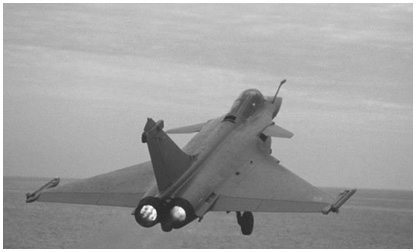
\includegraphics[width=.55\linewidth]{img_01}
}%figues de la page de garde


\def\xxpied{%
%Cycle 01 -- Modéliser le comportement des systèmes multiphysiques\\
\xxactivite%
}

\setcounter{secnumdepth}{5}
%---------------------------------------------------------------------------

\usepackage{pgfplots}
\begin{document}
%\defimages{images}
%\chapterimage{png/Fond_Cin}
\pagestyle{empty}


%%%%%%%% PAGE DE GARDE COURS
\ifcours
\begin{tikzpicture}[remember picture,overlay]
\node at (current page.north west)
{\begin{tikzpicture}[remember picture,overlay]
\node[anchor=north west,inner sep=0pt] at (0,0) {\includegraphics[width=\paperwidth]{\thechapterimage}};
\draw[anchor=west] (-2cm,-8cm) node [line width=2pt,rounded corners=15pt,draw=ocre,fill=white,fill opacity=0.6,inner sep=40pt]{\strut\makebox[22cm]{}};
\draw[anchor=west] (1cm,-8cm) node {\huge\sffamily\bfseries\color{black} %
\begin{minipage}{1cm}
\rotatebox{90}{\LARGE\sffamily\textsc{\color{ocre}\textbf{\xxnumpartie}}}
\end{minipage} \hfill
\begin{minipage}[c]{14cm}
\begin{titrepartie}
\begin{flushright}
\renewcommand{\baselinestretch}{1.1} 
\Large\sffamily\textsc{\textbf{\xxpartie}}
\renewcommand{\baselinestretch}{1} 
\end{flushright}
\end{titrepartie}
\end{minipage} \hfill
\begin{minipage}[c]{3.5cm}
{\large\sffamily\textsc{\textbf{\color{ocre} \discipline}}}
\end{minipage} 
 };
\end{tikzpicture}};
\end{tikzpicture}


\begin{tikzpicture}[overlay]
\node[shape=rectangle, 
      rounded corners = .25 cm,
	  draw= ocre,
	  line width=2pt, 
	  fill = ocre!10,
	  minimum width  = 2.5cm,
	  minimum height = 3cm,] at (18cm,0) {};
\node at (17.7cm,0) {\rotatebox{90}{\textbf{\Large\color{ocre}{\classe}}}};
%{};
\end{tikzpicture}

\vspace{3.5cm}

\begin{tikzpicture}[remember picture,overlay]
\draw[anchor=west] (-2cm,-6cm) node {\huge\sffamily\bfseries\color{black} %
\begin{minipage}{2cm}
\begin{center}
\LARGE\sffamily\textsc{\color{ocre}\textbf{\xxactivite}}
\end{center}
\end{minipage} \hfill
\begin{minipage}[c]{15cm}
\begin{titrechapitre}
\renewcommand{\baselinestretch}{1.1} 
\Large\sffamily\textsc{\textbf{\xxnumchapitre}}

\Large\sffamily\textsc{\textbf{\xxchapitre}}
\vspace{.5cm}

\renewcommand{\baselinestretch}{1} 
\normalsize\normalfont
\xxcompetences
\end{titrechapitre}
\end{minipage}  };
\end{tikzpicture}
\vfill

\begin{flushright}
\begin{minipage}[c]{.3\linewidth}
\begin{center}
\xxfigures
\end{center}
\end{minipage}\hfill
\begin{minipage}[c]{.6\linewidth}
\startcontents
\printcontents{}{1}{}
\end{minipage}
\end{flushright}

\begin{tikzpicture}[remember picture,overlay]
\draw[anchor=west] (4.5cm,-.7cm) node {
\begin{minipage}[c]{.2\linewidth}
\begin{flushright}

\includegraphics[width=2cm]{png/logoCC}
\end{flushright}
\end{minipage}
\begin{minipage}[c]{.2\linewidth}
\textsl{\xxauteur} \\
\textsl{\classe}
\end{minipage}
 };
\end{tikzpicture}
\newpage
\pagestyle{fancy}

\newpage
\pagestyle{fancy}

\else
\fi


%%%%%%%% PAGE DE GARDE TD
\iftd
%\begin{tikzpicture}[remember picture,overlay]
%\node at (current page.north west)
%{\begin{tikzpicture}[remember picture,overlay]
%\draw[anchor=west] (-2cm,-3.25cm) node [line width=2pt,rounded corners=15pt,draw=ocre,fill=white,fill opacity=0.6,inner sep=40pt]{\strut\makebox[22cm]{}};
%\draw[anchor=west] (1cm,-3.25cm) node {\huge\sffamily\bfseries\color{black} %
%\begin{minipage}{1cm}
%\rotatebox{90}{\LARGE\sffamily\textsc{\color{ocre}\textbf{\xxnumpartie}}}
%\end{minipage} \hfill
%\begin{minipage}[c]{13.5cm}
%\begin{titrepartie}
%\begin{flushright}
%\renewcommand{\baselinestretch}{1.1} 
%\Large\sffamily\textsc{\textbf{\xxpartie}}
%\renewcommand{\baselinestretch}{1} 
%\end{flushright}
%\end{titrepartie}
%\end{minipage} \hfill
%\begin{minipage}[c]{3.5cm}
%{\large\sffamily\textsc{\textbf{\color{ocre} \discipline}}}
%\end{minipage} 
% };
%\end{tikzpicture}};
%\end{tikzpicture}

%%%%%%%%%% PAGE DE GARDE TD %%%%%%%%%%%%%%%
%\begin{tikzpicture}[overlay]
%\node[shape=rectangle, 
%      rounded corners = .25 cm,
%	  draw= ocre,
%	  line width=2pt, 
%	  fill = ocre!10,
%	  minimum width  = 2.5cm,
%	  minimum height = 2.5cm,] at (18.5cm,0) {};
%\node at (17.7cm,0) {\rotatebox{90}{\textbf{\Large\color{ocre}{\classe}}}};
%%{};
%\end{tikzpicture}

% PARTIE ET CHAPITRE
%\begin{tikzpicture}[remember picture,overlay]
%\draw[anchor=west] (-1cm,-2.1cm) node {\large\sffamily\bfseries\color{black} %
%\begin{minipage}[c]{15cm}
%\begin{flushleft}
%\xxnumchapitre \\
%\xxchapitre
%\end{flushleft}
%\end{minipage}  };
%\end{tikzpicture}

% Bandeau titre exo
\begin{tikzpicture}[remember picture,overlay]
\draw[anchor=west] (-2cm,-6cm) node {\huge\sffamily\bfseries\color{black} %
\begin{minipage}{5cm}
\begin{center}
\LARGE\sffamily\color{ocre}\textbf{\textsc{\xxactivite}}

\begin{center}
\xxfigures
\end{center}

\end{center}
\end{minipage} \hfill
\begin{minipage}[c]{12cm}
\begin{titrechapitre}
\renewcommand{\baselinestretch}{1.1} 
\large\sffamily\textbf{\textsc{\xxtitreexo}}

\small\sffamily{\textbf{\textit{\color{black!70}\xxsourceexo}}}
\vspace{.5cm}

\renewcommand{\baselinestretch}{1} 
\normalsize\normalfont
\xxcompetences
\end{titrechapitre}
\end{minipage}  };
\end{tikzpicture}

\else
\fi


%%%%%%%% PAGE DE GARDE FICHE
\iffiche
\begin{tikzpicture}[remember picture,overlay]
\node at (current page.north west)
{\begin{tikzpicture}[remember picture,overlay]
\draw[anchor=west] (-2cm,-3.25cm) node [line width=2pt,rounded corners=15pt,draw=ocre,fill=white,fill opacity=0.6,inner sep=40pt]{\strut\makebox[22cm]{}};
\draw[anchor=west] (1cm,-3.25cm) node {\huge\sffamily\bfseries\color{black} %
\begin{minipage}{1cm}
\rotatebox{90}{\LARGE\sffamily\textsc{\color{ocre}\textbf{\xxnumpartie}}}
\end{minipage} \hfill
\begin{minipage}[c]{14cm}
\begin{titrepartie}
\begin{flushright}
\renewcommand{\baselinestretch}{1.1} 
\large\sffamily\textsc{\textbf{\xxpartie} \\} 

\vspace{.2cm}

\normalsize\sffamily\textsc{\textbf{\xxnumchapitre -- \xxchapitre}}
\renewcommand{\baselinestretch}{1} 
\end{flushright}
\end{titrepartie}
\end{minipage} \hfill
\begin{minipage}[c]{3.5cm}
{\large\sffamily\textsc{\textbf{\color{ocre} \discipline}}}
\end{minipage} 
 };
\end{tikzpicture}};
\end{tikzpicture}


\begin{tikzpicture}[overlay]
\node[shape=rectangle, 
      rounded corners = .25 cm,
	  draw= ocre,
	  line width=2pt, 
	  fill = ocre!10,
	  minimum width  = 2.5cm,
%	  minimum height = 2.5cm,] at (18.5cm,0.5cm) {};
	  minimum height = 2.5cm,] at (18.5cm,0.5cm) {};
\node at (17.7cm,0.5cm) {\rotatebox{90}{\textsf{\textbf{\large\color{ocre}{\classe}}}}};
%{};
\end{tikzpicture}



\else
\fi



\vspace{4cm}
\pagestyle{fancy}
\thispagestyle{plain}

\def\columnseprulecolor{\color{ocre}}
%\setlength{\columnseprule}{0.4pt} 

%\defimages2{images}



\section{Présentation}
\begin{multicols}{2}
Les propulseurs utilisés dans les applications militaires ou civiles subissent, avant leur mise en service, des tests de certification visant à contrôler leur bon fonctionnement et le respect des normes de sécurité.

Ces tests consistent à simuler au sol les conditions de vol subies par le propulseur et à observer les réactions de celui-ci consécutives à des commandes de pilotage.
	
La DGA (Direction Générale de l'Armement) dispose dans son centre d'essais des propulseurs, situé à Saclay, de bancs d'essais dédiés à la certification et à la mise au point de différents types de propulseurs d'avions ou de missiles. 

\subsection{Principe de fonctionnement d'un turboréacteur}
Un turboréacteur est un propulseur fonctionnant sur le principe d'action-réaction. La différence de vitesse entre l'air entrant et les gaz produits entraîne une variation de quantité de mouvement et donc un effort de poussée (voir \autoref{doc_01}  ci-dessous). 

L'air ambiant est conditionné à l'entrée puis comprimé à l'aide de compresseurs centrifuges à étages multiples. Le carburant est alors injecté dans la chambre de combustion, mélangé à l'air puis enflammé, ce qui produit ainsi l'énergie permettant l'accélération des gaz au passage de la tuyère d'éjection à ouverture variable. Leur passage dans une turbine permet en outre d'entraîner les étages de compression.

\begin{figure}[H]
\centering
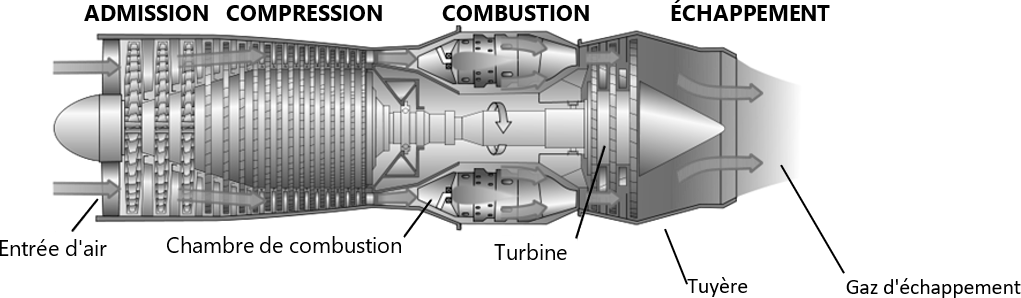
\includegraphics[width=.9\linewidth]{doc_01}
\caption{\label{doc_01} Structure d'un turboréacteur}
\end{figure}

\subsection{Le banc d'essais}
Un banc d'essais de turboréacteur est constitué de trois compartiments (voir \autoref{doc_02}).
	Le premier compartiment (A) est alimenté par une soufflerie et a pour fonction de conditionner le flux d'air en amont de la turbomachine testée. Il est ainsi possible de contrôler le débit, la température et la pression de l'air en admission.
	
	Le deuxième compartiment (B) contient le propulseur à tester. Celui-ci est maintenu par une structure porteuse permettant entre autres les mesures des efforts de poussée. Il est séparé du compartiment (A) par une cloison étanche munie d'un orifice permettant le passage de l'air calibré.  Le flux d'air peut alors être laissé libre en amont du réacteur ou guidé par un raccordement jusqu'à l'entrée de celui-ci, permettant ainsi des essais dits en << veine forcée >>. 
	
	Le troisième compartiment (C) permet la collecte et l'évacuation des gaz produits lors de la combustion. 
	
	La pression à l'intérieur du compartiment B est régulée afin de simuler différentes conditions d'altitude.
	
	Des vannes inter-compartiments permettent d'assurer une circulation d'air autour du réacteur afin de simuler le refroidissement externe du moteur en fonctionnement.
	
	La pression du compartiment A est ajustable de 0,05 à \SI{3}{bar}. Celle des compartiments B et C de 0,05 à \SI{1,05}{bar}. La température d'alimentation du compartiment A est variable de\SI{-56}{\degres C} à \SI{150}{\degres C}. La capacité de ventilation est réglable de 27 à \SI{40}{kg/s}. En réglant ces différents paramètres, il est possible de simuler sur ce type de banc l'ensemble des conditions d'utilisation d'un turboréacteur.

\begin{figure}[H]
\centering
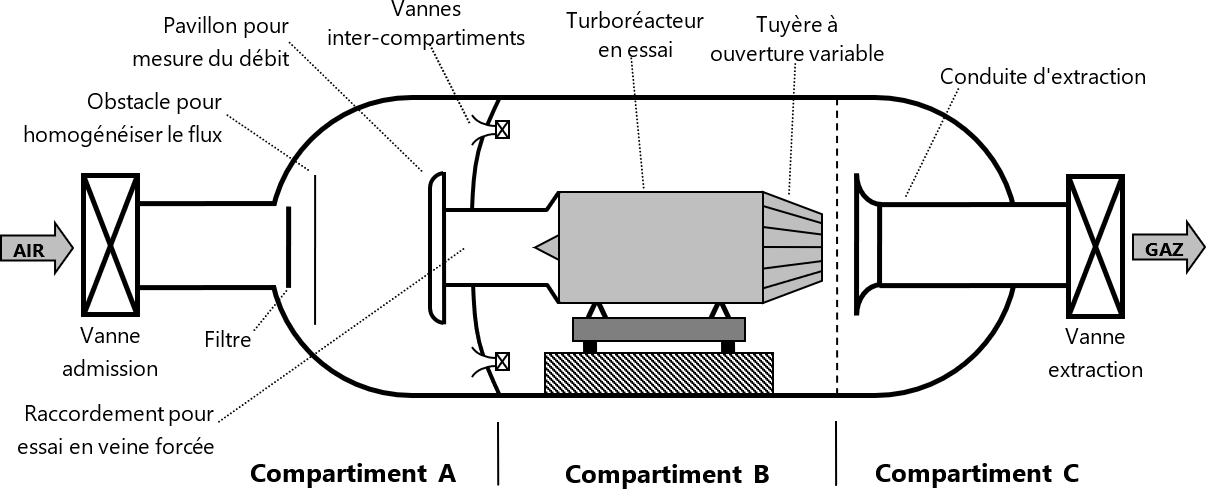
\includegraphics[width=.9\linewidth]{doc_02}
\caption{\label{doc_02} Structure d'un banc d'essais}
\end{figure}


\begin{figure}[H]
\centering
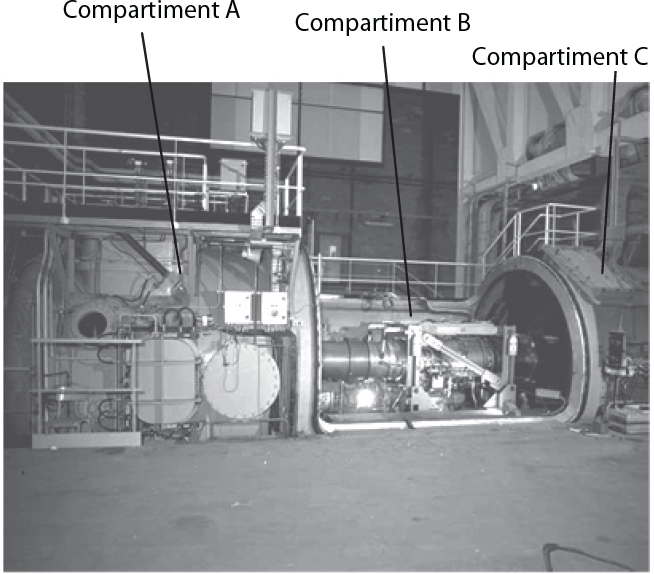
\includegraphics[width=.8\linewidth]{img_02}
\caption{\label{img_02} Vue d'ensemble du banc d'essais (compartiment B ouvert)}
\end{figure}

\begin{figure}[H]
\centering
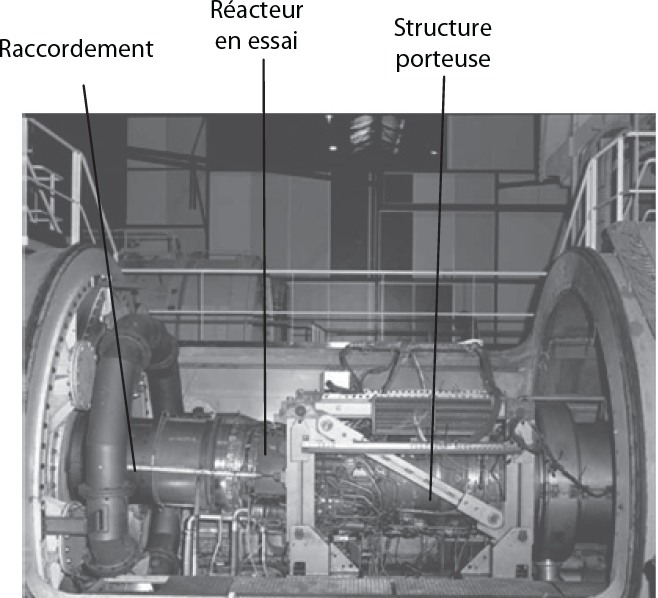
\includegraphics[width=.8\linewidth]{img_03}
\caption{\label{img_03} Vue du compartiment B}
\end{figure}


\subsection{Camibration du banc -- Réacteur simulé}
	Un banc d'essais nécessite pour fonctionner correctement une phase de calibration permettant d'affiner les réglages utilisés lors des tests et d'étalonner les appareils de mesures. On s'assure notamment dans cette phase que le compartiment A possède un comportement conforme aux besoins des tests.
	Les coûts en carburant et en matériel liés à l'utilisation d'un turboréacteur sont tels que, pour ces phases de calibration, les ingénieurs de la DGA ont imaginé une solution consistant à remplacer le propulseur réel par une structure simulant sa présence (voir \autoref{doc_03}).

\begin{figure}[H]
\centering
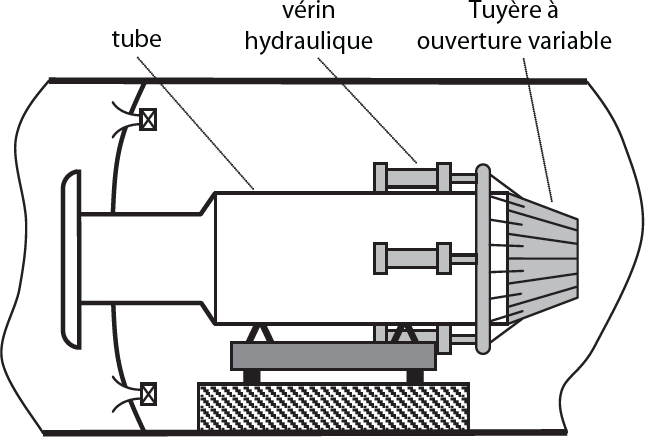
\includegraphics[width=.5\linewidth]{doc_03}
\caption{\label{doc_03} Réacteur simulé}
\end{figure}

	Cette structure est composée d'un tube représentant le corps du réacteur et d'une tuyère à ouverture variable actionnée par quatre vérins hydrauliques et permettant de faire varier la vitesse de l'air éjecté. On notera que dans ce cas, il n'y a pas de combustion interne au dispositif. Le tube est fixé sur la structure porteuse réelle avec les mêmes points d'encrage que le propulseur et est raccordé directement à la veine forcée. 

\subsection{Tuyère à ouverture variable}

La tuyère à ouverture variable montée sur le tube, en aval de l'écoulement, a pour fonction de faire varier la section de la veine de fluide en sortie de tube.
\begin{figure}[H]
\centering
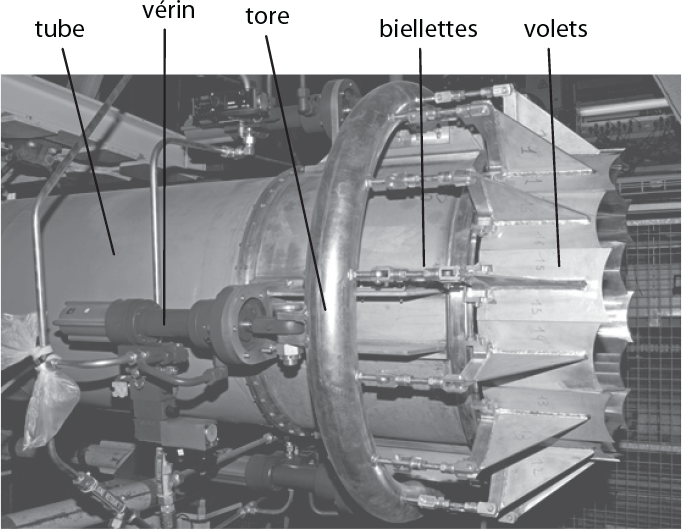
\includegraphics[width=.5\linewidth]{img_04}
\caption{\label{img_04}Tuyère à ouverture variable}
\end{figure}

	La solution imaginée consiste à disposer seize volets articulés sur la périphérie du tube qui permettent ainsi de réduire la section de passage du fluide (voir documents 4 et 5 ci-dessous). Ces volets sont mis en mouvement par seize biellettes toutes identiques reliées à une pièce de forme torique (tore) elle-même mise en translation par quatre vérins hydrauliques répartis régulièrement autour du tube.

Les commandes de ces vérins sont synchronisées et asservies en position. La DGA a confié la réalisation de cette commande à la société Bosch-Rexroth.


\begin{figure}[H]
\centering
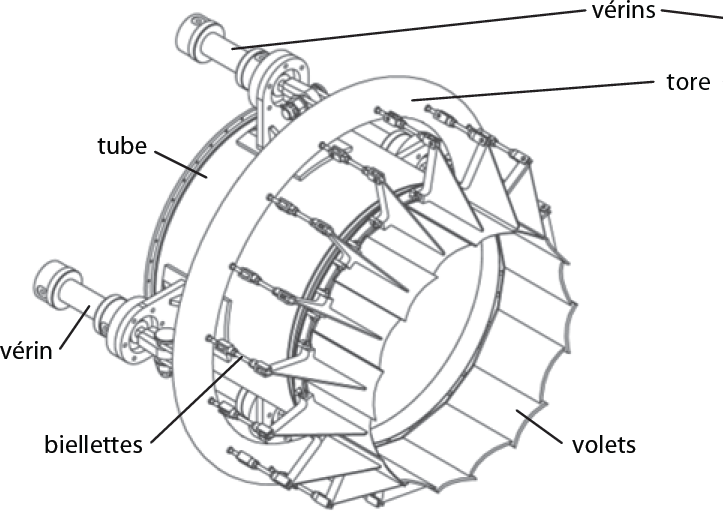
\includegraphics[width=.8\linewidth]{doc_04}
\caption{\label{doc_04}Tuyère ouverte}
\end{figure}

\begin{figure}[H]
\centering
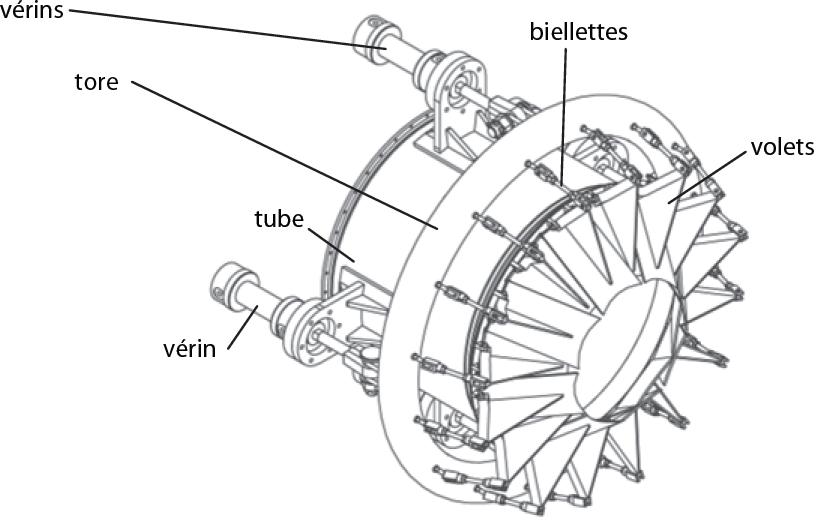
\includegraphics[width=.8\linewidth]{doc_05}
\caption{\label{doc_05} Tuyère fermée}
\end{figure}

	La consigne d'ouverture de la tuyère est élaborée au niveau de la console de pilotage. Elle est transmise à des modules de commande spécifiques à chaque vérin. Ceux-ci sont pilotés par des servo-distributeurs hydrauliques à commande électrique. Un contrôle de la position est effectué par un capteur à magnétostriction intégré dans le corps du vérin. Les caractéristiques de ces composants sont fournies en annexe 2.
	
\subsection*{Objectifs de l'étude proposée}
		On se propose dans ce sujet de valider les solutions choisies par les concepteurs vis-à-vis des performances attendues listées au cahier des charges.
		
\end{multicols}

\section{Modélisation de la chaîne fonctionnelle réalisant la fonction de service << faire varier le diamètre de la veine de fluide >> \label{sec_B}}

\begin{obj}
Cette partie a pour objectif de proposer un modèle de comportement pour les éléments constitutifs de la chaîne fonctionnelle réalisant la fonction de service. Cette modélisation permettra de valider une partie des performances attendues et de préparer la synthèse du correcteur pour la partie suivante.
\end{obj}

	Dans l'ensemble de cette partie, nous n'étudierons qu'une seule des 4 chaînes fonctionnelles constituant le système complet. Nous ferons l'hypothèse que les chaînes sont parfaitement identiques et que la charge est également répartie sur chacun des 4 vérins.
	
	On donne ci-dessous un extrait du cahier des charges relatif à la fonction de service.

\begin{figure}[H]
\centering
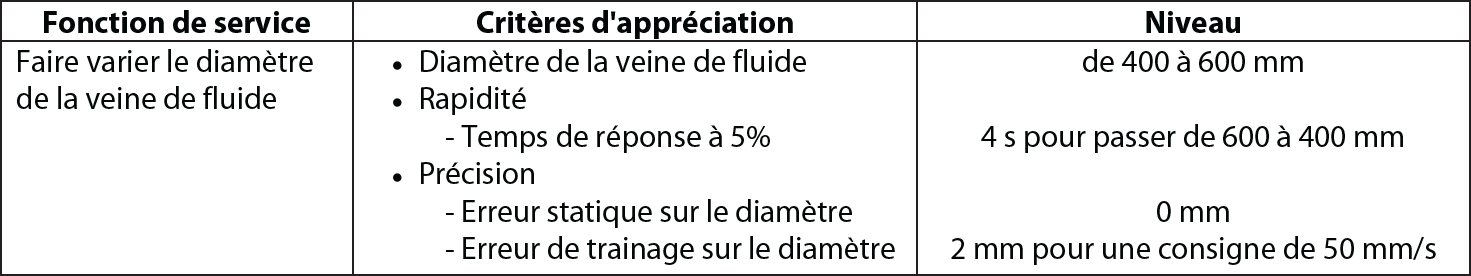
\includegraphics[width=\linewidth]{img_05}
%\caption{\label{doc_05} Tuyère fermée}
\end{figure}

	 Le schéma-bloc adopté pour la modélisation de cette chaîne est le suivant.
\begin{figure}[H]
\centering
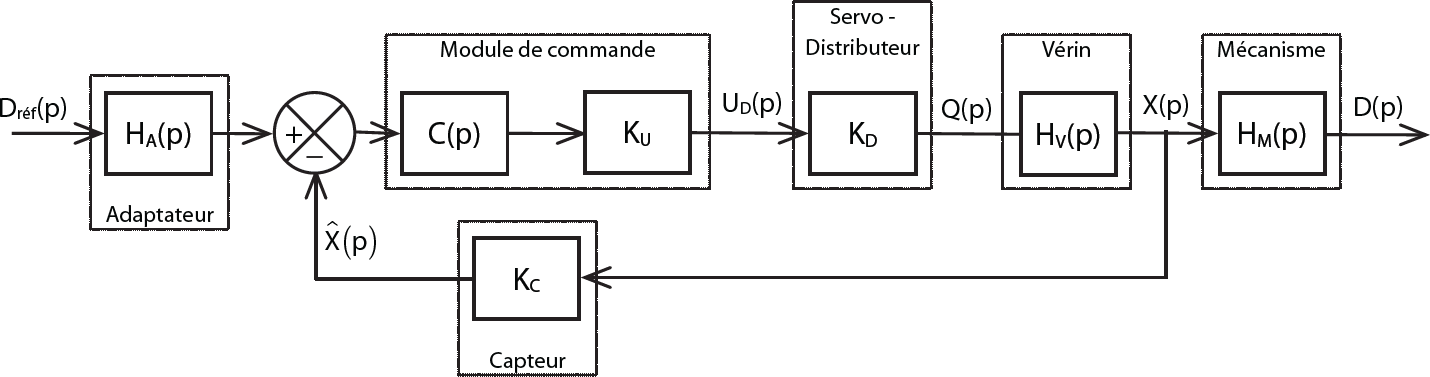
\includegraphics[width=\linewidth]{img_06}
%\caption{\label{doc_05} Tuyère fermée}
\end{figure}	 


\noindent Notations :

\noindent Grandeurs physiques :
\begin{itemize}
\item $D_{\text{ref}}(p)$ : 	diamètre de consigne de la section d'ouverture de la tuyère;
\item $U_D(p)$	 	:	tension de commande du servo-distributeur hydraulique;
\item $Q(p)$	  	:	débit volumique de commande du vérin;
\item $X(p)$	 	:	déplacement de la tige du vérin;
\item $\hat{X}(p)$ 	:	estimation du déplacement par le capteur;
\item $D(p)$		:	diamètre de la section d'ouverture de la tuyère.
\end{itemize}

\noindent Fonctions de transfert et gains :
\begin{itemize}
\item $H_A(p)$	: 	fonction de transfert du bloc d'adaptation permettant de traduire la consigne;
\item $C(p)$	: 	fonction de transfert du correcteur de la chaîne de commande;
\item $K_U$	: 	gain du convertisseur numérique analogique;
\item $K_D$	:	gain du servo-distributeur hydraulique;
\item $K_C$	:	gain du capteur de déplacement;
\item $H_V(p)$	:	fonction de transfert du vérin hydraulique;
\item $H_M(p)$	:	fonction de transfert du mécanisme de transmission de mouvement de la tige jusqu'aux volets.
\end{itemize}

Conventions d'écriture et hypothèses :

	Par convention, nous noterons $F(p)$ l'image par la transformation de Laplace d'une fonction du temps $f(t)$ où $p$ symbolise la variable de Laplace.

	En l'absence de précisions complémentaires, le comportement des composants sera supposé en première approximation linéaire, continu et invariant. On se place par ailleurs dans l'hypothèse des conditions d'Heaviside validées.

Les données fournies par le capteur sont numériques, tout comme les signaux traités dans la chaîne d'information. La période d'échantillonnage est suffisamment faible pour être négligeable devant la dynamique globale du système. Les différentes variables seront donc toutes considérées comme des fonctions continues du temps. 


\subsection{Modélisation du comportement cinématique du mécanisme\label{sec_B1}}

\begin{obj}
Il s'agit dans un premier temps de valider la linéarité du comportement du mécanisme de transformation de mouvement en établissant la loi de comportement cinématique et d'établir les performances de la chaîne de commande des vérins permettant le respect du cahier des charges.
\end{obj}

	L'annexe \ref{ann_03} montre le mécanisme de transformation du déplacement $x(t)$ d'un vérin en rotation $\alpha(t)$ d'un volet dans les positions extrêmes : tuyère pleine ouverture (figure 4) et tuyère ouverture réduite (figure 5).
	
\noindent Notations et hypothèses :
	
	On suppose que le mécanisme étudié admet le plan  $\left(O,\vect{x_1}, \vect{y_1}\right)$ comme plan de symétrie géométrique.
Le modèle cinématique adopté est précisé par le schéma cinématique de la figure 6 (annexe \ref{ann_03}). 
Les données géométriques et une figure de changement de bases sont fournies avec la figure 7 (annexe \ref{ann_03}). 
La position initiale est définie par $x(0)=\SI{0}{mm}$
$\alpha(0) = 0\degres$.

%Q4
\subparagraph{}\textit{Écrire la relation vectorielle traduisant la fermeture géométrique de la chaîne de solides. En déduire les deux équations scalaires en projection dans la base  $\left( \vect{x_1};\vect{y_1} \right)$.}

%Q5
\subparagraph{\label{q_05}}\textit{En éliminant l'inconnue $\beta$, exprimer $\alpha$ en fonction de $x$. Puis le diamètre $D$ de la veine fluide en fonction de $\alpha$ et $D_0$ le diamètre initial de la tuyère.}

%Q6
\subparagraph{}\textit{On donne annexe \ref{ann_03} figure 8 le tracé de la fonction $D(x)$ déduite de la question précédente. Peut-on linéariser cette fonction sur cet intervalle ? Si oui, proposer une expression affine de $D$ en fonction de $x$. }

% Q7
\subparagraph{}\textit{À partir du résultat de la question précédente, déduire du cahier des charges relatif à la fonction de service les niveaux des critères à valider pour la commande des vérins (course, temps de réponse, précision).}

\subsection{Modélisation du comportement du servo-distributeur hydraulique}

\begin{obj}
Il s'agit ici d'établir un modèle de comportement du servo-distributeur et de valider les choix des composants hydrauliques vis-à-vis du cahier des charges.
\end{obj}

La fonction de distribution de l'énergie est assurée par un servo-distributeur dont les caractéristiques principales sont données en annexe \ref{ann_02}.
% Q8
\subparagraph{}\textit{À partir de la courbe de débit et des caractéristiques fournies, proposer une valeur numérique pour le gain $K_D$ du servo-distributeur (on négligera pour cela la légère non linéarité perceptible sur la courbe).   }

% Q9
\subparagraph{}\textit{Calculer la vitesse maximale $V_{\text{max}}$ (en \si{m/s}) de déplacement de la tige du vérin. Vérifier alors que les performances maximales des composants hydrauliques choisis sont compatibles avec les exigences de rapidité spécifiées au cahier des charges.   }

\subsection{Modélisation du comportement du capteur de déplacement}

\begin{obj}
Établir un modèle de comportement du capteur de déplacement et valider les performances du capteur vis-à-vis du cahier des charges.
\end{obj}

Le vérin hydraulique inclut un capteur de position fonctionnant sur le principe de la magnétostriction et dont les principales caractéristiques sont données en annexe \ref{ann_02}.

Le signal fourni par ce capteur est numérique. La mesure s'effectue comme sur un codeur incrémental par incrémentation des tops émis par le composant. L'estimation $\hat{x}(t)$ du déplacement $x(t)$  correspond au nombre de tops émis lors de ce déplacement.


% Q10
\subparagraph{}\textit{En tenant compte de la résolution du capteur, donner la valeur numérique du gain $K_C$ du capteur.   }

% Q11
\subparagraph{}\textit{Donner la valeur maximale prise par $\hat{x}(t)$ lors du déplacement du vérin. Combien de bits sont nécessaires pour coder cette information ? Est-ce compatible avec le capteur choisi ?   }

% Q12
\subparagraph{}\textit{Quelle est la spécificité du code Gray ? En quoi est-elle intéressante pour une mesure par incrémentation ? }

\subsection{Modélisation du comportement du vérin -- Hypothèse fluide incompressible}

\begin{obj}
Il s'agit dans cette partie de proposer un premier modèle du comportement du vérin en adoptant une hypothèse de fluide incompressible.
\end{obj}

Le résultat de la partie précédente nous permet de réduire l'étude à la commande en position du vérin. Nous adopterons pour cela le schéma-bloc suivant où $X_{\text{réf}}(p)$ représente la consigne de position du vérin équivalente à la consigne portant sur le diamètre de la veine de fluide.

\begin{figure}[H]
\centering
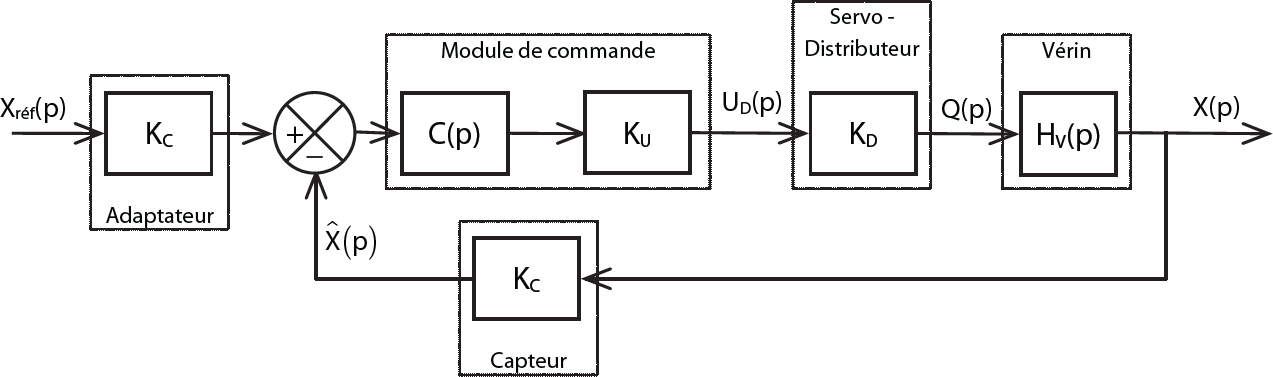
\includegraphics[width=\linewidth]{img_07}
%\caption{\label{doc_05} Tuyère fermée}
\end{figure}


Dans toute cette partie, on prendra  $K_U = \SI{5e-4}{V}$.
Nous considérerons par ailleurs une action proportionnelle du correcteur telle que  $C(p)=K_P$.
Nous nous proposons en première approximation de considérer le fluide utilisé (huile) comme étant incompressible. Cette hypothèse induit la relation suivante : $q(t)=S\dfrac{\dd x(t)}{\dd t}$,  où $S$ représente la section utile du vérin en sortie de tige.


% Q13
\subparagraph{}\textit{Donner l'expression de la fonction de transfert du vérin  $H_v(p)=\dfrac{X(p)}{Q(p)}$. }

% Q14
\subparagraph{}\textit{Donner alors l'expression de la fonction de transfert en boucle fermée $H_{\text{BF}}(p)=\dfrac{X(p)}{X_{\text{réf}}(p)}$. La mettre sous la forme $F(p)=\dfrac{1}{1+Tp}$  en précisant les expressions de $K$ et de $T$.}

% Q15
\subparagraph{}\textit{Quelle est alors l'écart de position consécutif à une consigne de \SI{100}{mm} ? Est-ce compatible avec la performance spécifiée dans le cahier des charges ?}

\subsection{Modélisation du comportement du vérin -- Hypothèse fluide compressible}

\begin{obj}
Il s'agit ici de proposer un modèle plus affiné du comportement du vérin en tenant compte de la compressibilité du fluide et du comportement dynamique du mécanisme.
\end{obj}

L'hypothèse d'incompressibilité formulée dans la partie précédente conduit à un modèle cinématique qui ne tient pas compte des causes du mouvement. Pour rendre compte du comportement dynamique du système il faut modifier le modèle de comportement du vérin en tenant compte de la compressibilité du fluide.

L'évolution du débit est alors une fonction du déplacement mais aussi de la pression sous la forme de la relation suivante :

$$ 
[1] \quad q(t)= S\dfrac{\dd x(t)}{\dd t} + \dfrac{V_0}{B} \dfrac{\dd \sigma(t) }{\dd t}
\quad \text{avec} 
\left\{
\begin{array}{ll}
\sigma(t) &\text{: pression utile dans le vérin.}  \\ 
& \text{    On notera }\Sigma(p)\text{ sa transformée de Laplace;}\\
V_0 &\text{: demi volume de fluide contenu dans le vérin;} \\
B &\text{: coefficient de compressibilité du fluide.}
\end{array}
\right. .
$$

La pression utile induit l'effort développé par le vérin que nous noterons $F_v$ tel que :
$[2] \quad F_v(p) = S\Sigma(p)$, où $S$ représente la section utile du vérin en sortie de tige.
C'est cette action qui permet la mise en mouvement du mécanisme et par conséquent celui des volets. 

\subsubsection{Modélisation du comportement dynamique du mécanisme  }
\begin{obj}
On cherche à déterminer la masse équivalente $M_{\text{eq}}$, ramenée à la tige du vérin, du mécanisme de transformation de mouvement actionné par un vérin, c'est-à-dire un mécanisme réduit au quart de l'ensemble composé du tore, des 16 biellettes et des 16 volets.
\end{obj}

Le calcul sera effectué sur un seul des ensembles bielle-volet puis multiplié par 4 pour obtenir le résultat valable pour un vérin. A l'inverse on considérera qu'un vérin déplace un quart de la masse du tore. On adopte pour ce mécanisme le modèle utilisé pour la partie B1 et donné par son schéma cinématique sur la figure 6 de l'annexe \ref{ann_03}.

\paragraph*{Notations et hypothèses}
On suppose que le mécanisme étudié admet le plan $\left(O,\vect{x_1}, \vect{y_1}\right)$ comme plan de symétrie géométrique. On néglige la masse des biellettes devant celle du tore et des volets. Les solides sont supposés homogènes. Le référentiel associé au bâti \textbf{1} est supposé galiléen.

Le modèle cinématique adopté est précisé par le schéma cinématique de la figure 6 de l'annexe \ref{ann_03}. Les données géométriques et une figure de changement de bases sont fournies avec la figure 7 de l'annexe \ref{ann_03}.

Avant de rechercher la masse équivalente, on se propose d'estimer les caractéristiques d'inertie d'un volet. Le modèle à géométrie simplifiée donné par la  figure 9 de l'annexe \ref{ann_04} fait apparaître que le volet peut être décrit par l'assemblage de 3 volumes élémentaires numérotés 1, 2 et 3. On suppose que la contribution du volume 3 aux caractéristiques d'inertie d'un volet est négligeable.


% Q17
\subparagraph{}\textit{Déterminer, avec les hypothèses précédentes, le moment d'inertie par rapport à l'axe $\left(C,\vect{z}\right)$ note $I_{\left(V,Cz\right)}$ d'un volet en fonction de la masse volumique $\rho$ et des caractéristiques géométriques $H$, $L$, $d$, $a$ et $e$.}

% Q18
\subparagraph{}\textit{Exprimer l'énergie cinétique galiléenne de l'ensemble de solides \textbf{(3+4+5)} en fonction de $M_t$, $I_{\left(V,Cz\right)}$ , $\dot{\alpha}$  et~$\dot{x}$.}

% Q19
\subparagraph{}\textit{La  figure 11 de l'annexe \ref{ann_04} donne la variation de l'angle $\alpha$ en fonction de $x$ obtenue à la question \ref{q_05}. On cherche à linéariser la loi de variation sous la forme $\alpha=-k_1 x$. Donner la valeur de $k_1$ en précisant son unité.}

% Q20
\subparagraph{}\textit{Après avoir précisé la méthode utilisée pour définir la masse équivalente recherchée, exprimer la masse équivalente $M_{\text{eq}}$ en fonction de $M_t$,  $I_{\left(V,Cz\right)}$ et $k_1$. }

% Q21
\subparagraph{}\textit{Faire l'application numérique pour $M_t=\SI{22}{kg}$ et $I_{\left(V,Cz\right)}=\SI{8e4}{kg.mm^2}$. }

On donne (question \ref{q_22}) un schéma-bloc modélisant le comportement du vérin avec l'hypothèse d'un fluide compressible. Sur ce schéma, $V(p)$ représente l'image par la transformation de Laplace de la vitesse de translation $v(t)$ de la tige du vérin. 
En considérant les actions de pesanteur négligeables et en se plaçant dans une phase de test à vide (sans flux d'air), l'application des lois de la dynamique donne la relation suivante : $[3] \quad  F_v(t)=M_{\text{eq}}\dfrac{\dd^2 x(t)}{\dd t^2}$.
  	 	 


% Q22
\subparagraph{\label{q_22}}\textit{À partir des équations [1], [2] et [3], recopier et compléter le schéma-blocs suivant en indiquant les fonctions de transferts de chaque bloc.}

\begin{figure}[H]
\centering
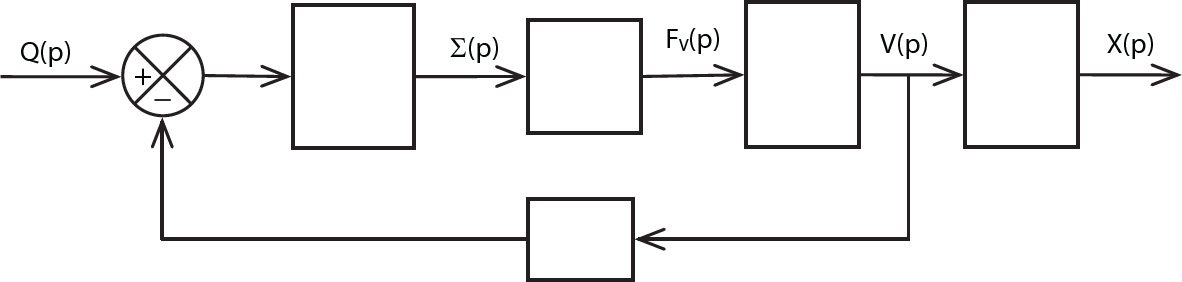
\includegraphics[width=.8\linewidth]{dr_Q22}
%\caption{\label{doc_05} Tuyère fermée}
\end{figure}


\subsubsection{Prise en compte de l'action de l'air sur les volets }

\begin{obj}
On cherche à déterminer l'action mécanique résistante équivalente $F_R$, ramenée à la tige du vérin, représentant les actions mécaniques de l'air sur les volets associés à un vérin, c'est-à-dire 4 des 16 volets.
\end{obj}


Le calcul sera effectué sur un seul des ensembles bielle-volet puis multiplié par 4 pour obtenir le résultat valable pour un vérin. On adopte pour ce mécanisme le modèle utilisé pour la partie \ref{sec_B1} et donné par son schéma cinématique sur la figure 6 de l'annexe \ref{ann_03}.


\paragraph*{Notations et hypothèses}
On suppose que le mécanisme étudié admet le plan $\left(O,\vect{x_1}, \vect{y_1}\right)$ comme plan de symétrie géométrique. On néglige la masse des biellettes devant celle du tore et des volets. Les liaisons sont supposées parfaites. Le référentiel associé au bâti 1 est supposé galiléen.

Le modèle cinématique adopté est précisé par le schéma cinématique de la figure 6 de l'annexe \ref{ann_03}. Les données géométriques et une figure de changement de bases sont fournies avec la figure figure 7 de l'annexe \ref{ann_03}.

L'action de l'air sur un volet est assimilée à un glisseur $\torseurstat{F}{\text{air}}{5} = \torseurl{F_a\vect{y_5}}{\vect{0}}{K}$ dont l'axe central passe par le centre de poussée $K$ tel que  $\vect{CK}=c\vect{x_5}$.

L'action de la pression d'huile sur la tige du vérin est assimilée à un glisseur 
$\torseurstat{F}{\text{p}}{3} = \torseurl{F_v\vect{x_3}}{\vect{0}}{A}$ dont l'axe central passe par le centre de poussée $A$.


% Q23
\subparagraph{}\textit{Exprimer la puissance galiléenne développée par les actions mécaniques extérieures et intérieures à l'ensemble de solides \textbf{(3+4+5)} en fonction de $F_a$, $F_V$, $c$, $\dot{\alpha}$ et  $\dot{x}$. Montrer qu'elle peut se mettre sous la forme : $F_V - F_{\text{eq}}\dot{x}$  où $F_{\text{eq}}$ représente l'action équivalente de l'air sur un seul volet ramenée sur l'axe du vérin. On donnera alors l'expression de $F_{\text{eq}}$ en fonction $F_a$, $c$ et $k_1$.}

% Q24
\subparagraph{}\textit{En première approximation, on suppose que $F_a$ est de la forme $F_a = -k_2 \alpha$. Exprimer $F_R$ en fonction $c$, $k_1$, $k_2$ et $x$. On rappelle que $F_R$ est l'action mécanique résistante équivalente pour quatre volets. Mettre le résultat sous la forme $F_R = K_F x$  et donner l'expression de $K_F$.}

% Q25
\subparagraph{}\textit{Calculer la valeur numérique de $K_F$ avec $k_2 = \dfrac{15}{4} \times 10^3 \si{N/rad}$ et $c=\SI{200}{mm}$ .}

% Q26
\subparagraph{}\textit{Écrire le théorème de la résultante dynamique appliquée au solide \textbf{3} dans son mouvement par rapport à \textbf{1} en projection sur $\vect{x_1}$, comme s'il était seul en remplaçant l'ensemble des quatre groupes de solides \textbf{4} et \textbf{5} par les caractéristiques équivalentes déterminées précédemment. }

% Q27
\subparagraph{}\textit{Compléter le schéma-blocs en indiquant les fonctions de transfert de chaque bloc.}

\begin{figure}[H]
\centering
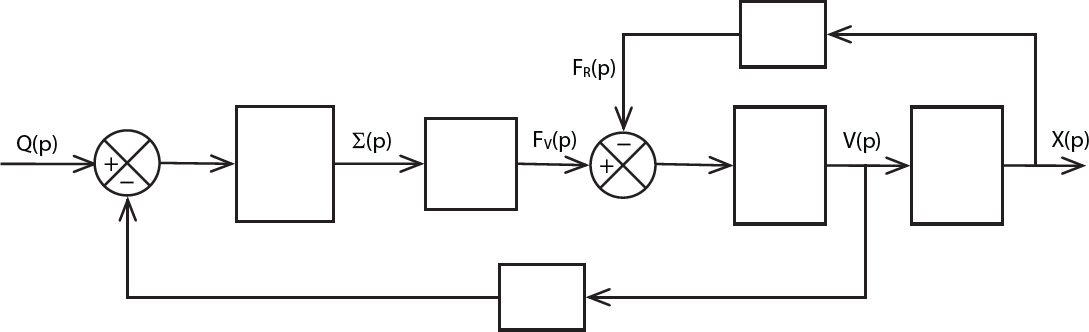
\includegraphics[width=.8\linewidth]{dr_Q27}
%\caption{\label{doc_05} Tuyère fermée}
\end{figure}


% Q28
\subparagraph{\label{q_28}}\textit{Donner l'expression de la fonction de transfert du vérin ainsi modélisé $H_v(p)=\dfrac{X(p)}{Q(p)}$. On donnera le résultat sous la forme suivante : $H_v(p)=\dfrac{K_v}{p\left(1+a_2 p^2\right)}$  en précisant les expressions de $K_V$ et $a_2$.}

\subsubsection{Validation du modèle de comportement du vérin}

Afin de valider le modèle établi, on se propose d'étudier le comportement en boucle fermée de la chaîne fonctionnelle de commande du vérin. On rappelle ci-dessous le schéma-bloc retenu et on considérera une correction proportionnelle telle que  $C(p)=K_p$.

\begin{figure}[H]
\centering
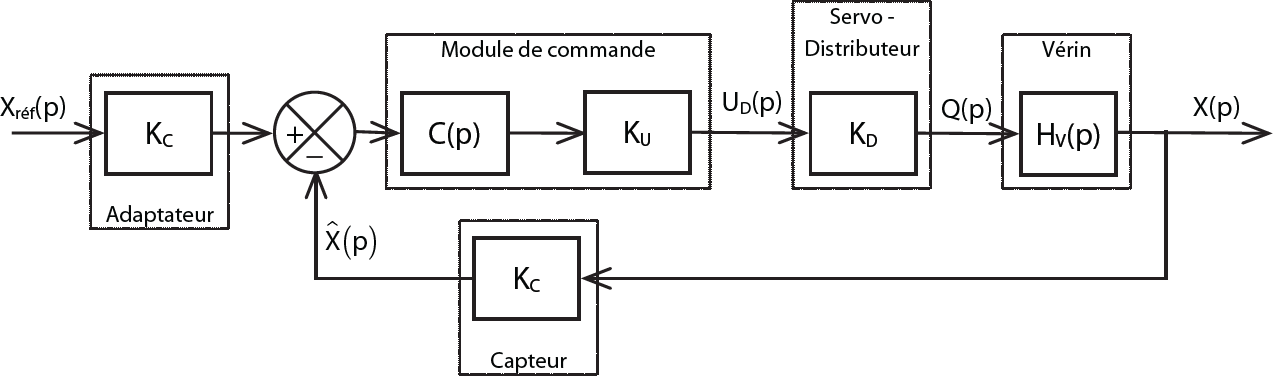
\includegraphics[width=\linewidth]{img_08}
%\caption{\label{doc_05} Tuyère fermée}
\end{figure}

% Q29
\subparagraph{}\textit{Donner l'expression de la forme canonique de la foncti0on de transfert en boucle fermée $H_{\text{BF}}=\dfrac{X(p)}{X_{\text{ref}}(p)}$. On donnera le résultat en fonction de $K_C$, $K_U$, $K_D$, $K_p$, $K_V$ et $a_2$. }


\vspace{.5cm}
% Q30
On donne une approximation des pôles de la FTBF : $p_1 = -5,50321\times 10^-6$, $p_{2,3} = 2,75161\times 10^{-6} \pm 4.76592\times 10^{-6} j$.

\subparagraph{}\textit{Discuter de la stabilité du système ainsi modélisé. Conclure sur le modèle de comportement du vérin établi en question \ref{q_28}.}

\subsubsection{Prise en compte d'un débit de fuite}

Pour pallier le problème de stabilité du modèle précédemment établi, une solution possible consiste à un introduire un débit de fuite entre les deux chambres du vérin. Celui-ci a pour effet de réduire artificiellement le débit réel entrant dans le vérin en fonction de la pression utile. Ce débit vaut alors : $q(t)-\delta \sigma(t)$  où $\delta$ est le coefficient de débit de fuite.

% Q31
\subparagraph{}\textit{Proposer une modification du schéma-blocs donné ci-dessous afin de prendre en compte le débit de fuite entre les chambres du vérin.  }

\begin{figure}[H]
\centering
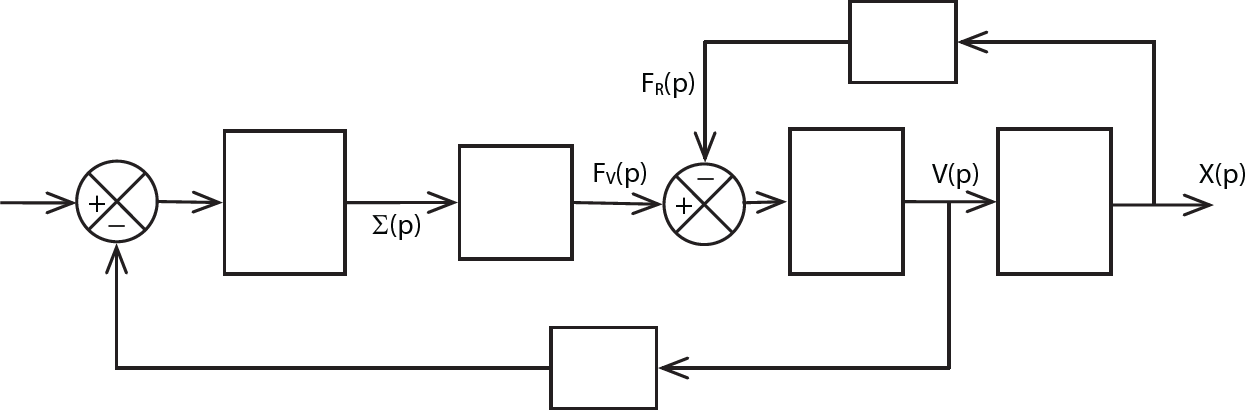
\includegraphics[width=.7\linewidth]{dr_Q31}
%\caption{\label{doc_05} Tuyère fermée}
\end{figure}



% Q32
\subparagraph{}\textit{Donner l'expression de la fonction de transfert du vérin ainsi modélisé  $H_v(p)=\dfrac{X(p)}{Q(p)}$. On donnera le résultat sous la forme suivante : $H_v(p)= \dfrac{K_V}{1+a_1p + a_2p^2 + a_3 p^3}$ en précisant les expressions de $K_V$, $a_1$, $a_2$ et $a_3$.}

\section{Synthèse du correcteur de la commande en position d'un vérin}
\begin{obj}
Cette partie a pour objectif de choisir et de régler le correcteur de la chaîne fonctionnelle assurant la fonction de service.
\end{obj}

	On donne ci-dessous un extrait du cahier des charges relatif à la fonction de service.
	

\begin{figure}[H]
\centering
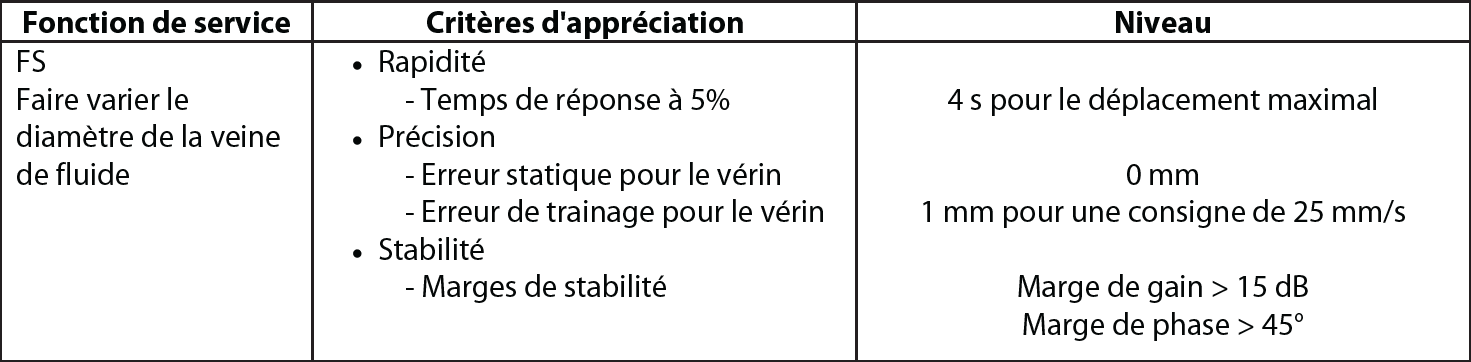
\includegraphics[width=\linewidth]{img_09}
%\caption{\label{doc_05} Tuyère fermée}
\end{figure}

	Afin de simplifier l'étude et en reprenant les résultats de la partie \ref{sec_B}, nous adopterons dans cette partie le schéma-bloc suivant pour modéliser la chaîne fonctionnelle.
	
	\begin{figure}[H]
\centering
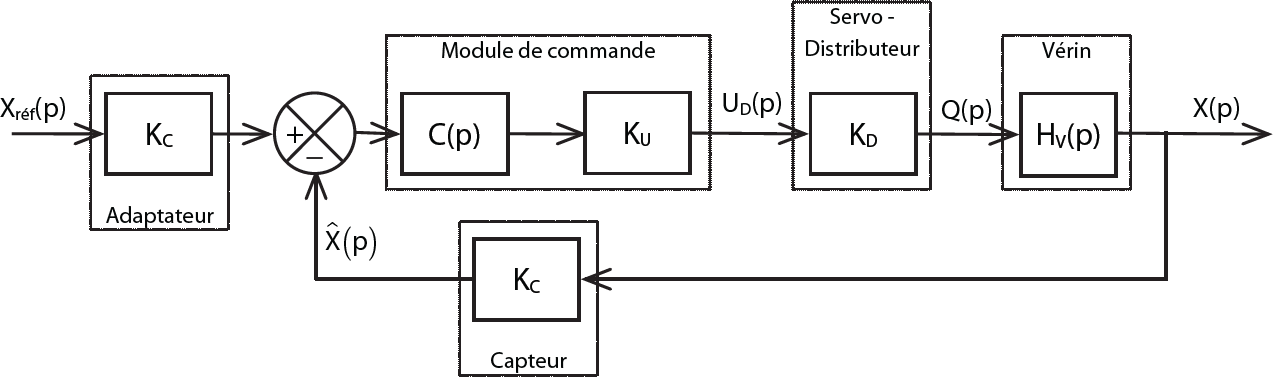
\includegraphics[width=\linewidth]{img_10}
%\caption{\label{doc_05} Tuyère fermée}
\end{figure}

\paragraph*{Notations}

Grandeurs physiques :
\begin{itemize}
\item $X_{\text{ref}}(p)$	: diamètre de consigne de la section d'ouverture de la tuyère;
\item $U_D(p)$		: tension de commande du servo-distributeur hydraulique;
\item $Q(p)$	  	: débit de fluide fourni par le servo-distributeur au vérin;
\item $X(p)$ 		: déplacement de la tige du vérin;
\item $\hat{X}(p)$ 	: estimation du déplacement par le capteur.
\end{itemize}

Fonctions de transfert et gains :
\begin{itemize}
\item $C(p)$	: fonction de transfert du correcteur de la chaîne de commande;
\item $K_U$	: gain du convertisseur numérique analogique;
\item $K_D$	: gain du servo-distributeur hydraulique;
\item $K_C$	: gain du capteur de déplacement;
\item $H_V(p)$	: fonction de transfert du vérin hydraulique.
\end{itemize}

\paragraph*{Valeurs numériques}
Indépendamment des résultats obtenus dans la partie B, nous prendrons les valeurs numériques suivantes :  
$K_C = \SI{2e5}{m^{-1}}$; 
$K_U = \SI{5e-4}{V}$ et 
$K_D = \SI{1e-5}{m^3.s^{-1}.V^{-1}}$.

\subsection{Modélisation de la boucle ouverte non corrigée}

\begin{obj}
Il s'agit ici de proposer un modèle du comportement en boucle ouverte non corrigée de la chaîne fonctionnelle.
\end{obj}

On donne  sur le document réponse (question \ref{q_33}) la représentation dans le plan de Bode de la fonction de transfert $H_V(p)$.
	
% Q33
\subparagraph{\label{q_33}}\textit{Proposer à partir du tracé du document réponse, une expression pour la fonction de transfert $H_V(p)$. On justifiera la réponse en traçant les diagrammes asymptotiques correspondants et en déterminant tous les coefficients utiles. On précise que les coefficients ont été choisis afin d'optimiser la rapidité du vérin.  }




% Q34
\subparagraph{}\textit{En déduire la valeur du gain statique en boucle ouverte non corrigée du système. On notera ce terme $K_{\text{BONC}}$. Tracer en rouge, sur le Bode de la question \ref{q_33}, le diagramme de la fonction de transfert en boucle ouverte du système complet non corrigé.  }

\subsection{Analyse des performances en correction proportionnelle}

\begin{obj}
Il s'agit ici d'analyser les performances de la commande en correction proportionnelle et de vérifier son adéquation au cahier des charges.
\end{obj}

Considérons dans un premier temps une correction proportionnelle telle que  $C(p)=K_P$.

% Q35
\subparagraph{}\textit{Donner l'ordre et la classe du système ainsi corrigé.  }

% Q36
\subparagraph{}\textit{Pour $K_P = 10$, donner les valeurs de l'erreur statique pour une consigne de \SI{100}{mm} et de l'erreur de traînage pour une consigne de vitesse de \SI{25}{mm/s}.  Le système peut-il répondre aux exigences de précision du cahier des charges ?}

% Q37
\subparagraph{}\textit{Le système comporte-t-il un risque d'instabilité ? Si oui, préciser pour quelle valeur de $K_p$ l'instabilité est possible (on attend une méthode graphique et un résultat sous la forme d'une puissance de 10). Conclure.}

\subsection{Réglage d'une correction proportionnelle et intégrale}
\begin{obj}
Il s'agit ici de proposer un réglage pour une correction proportionnelle et intégrale afin de satisfaire aux performances du cahier des charges.
\end{obj}
On prendra dans cette partie $C(p)=K_i \left(1+ \dfrac{1}{T_i p}\right)$.
% Q38
\subparagraph{}\textit{Tracer une représentation dans le plan de Bode de la fonction $C(p)$. On demande le diagramme asymptotique ainsi que l'allure des courbes réelles.}

% Q39
\subparagraph{}\textit{Donner l'ordre et la classe du système ainsi corrigé.  }

Afin de garantir au système une réactivité optimale, on choisit de régler la constante de temps $T_i$ permettant de compenser le mode le plus lent du système non corrigé.
% Q40
\subparagraph{}\textit{Quelle valeur de $T_i$ permet de compenser le mode le plus lent du système non corrigé ?  }

% Q41
\subparagraph{}\textit{Tracer le diagramme de Bode de la fonction de transfert en boucle ouverte du système ainsi corrigé pour  $K_i = 1$ (asymptotes et allures des courbes réelles).}

% Q42
\subparagraph{}\textit{Quelle valeur de $K_i$ garantit les exigences de précision du cahier des charges ?}

% Q43
\subparagraph{}\textit{Estimer pour cette valeur les marges de gain et de phase du système et conclure sur le choix de cette correction. On pourra prendre une valeur approchée de $K_i$ et on rappelle, si besoin, que  $\log 2 \simeq 0,3$.}

\section{Annexes}
\subsection{\label{ann_02}Composants de la chaîne fonctionnelle de commande d'un vérin}
\begin{figure}[H]
\centering
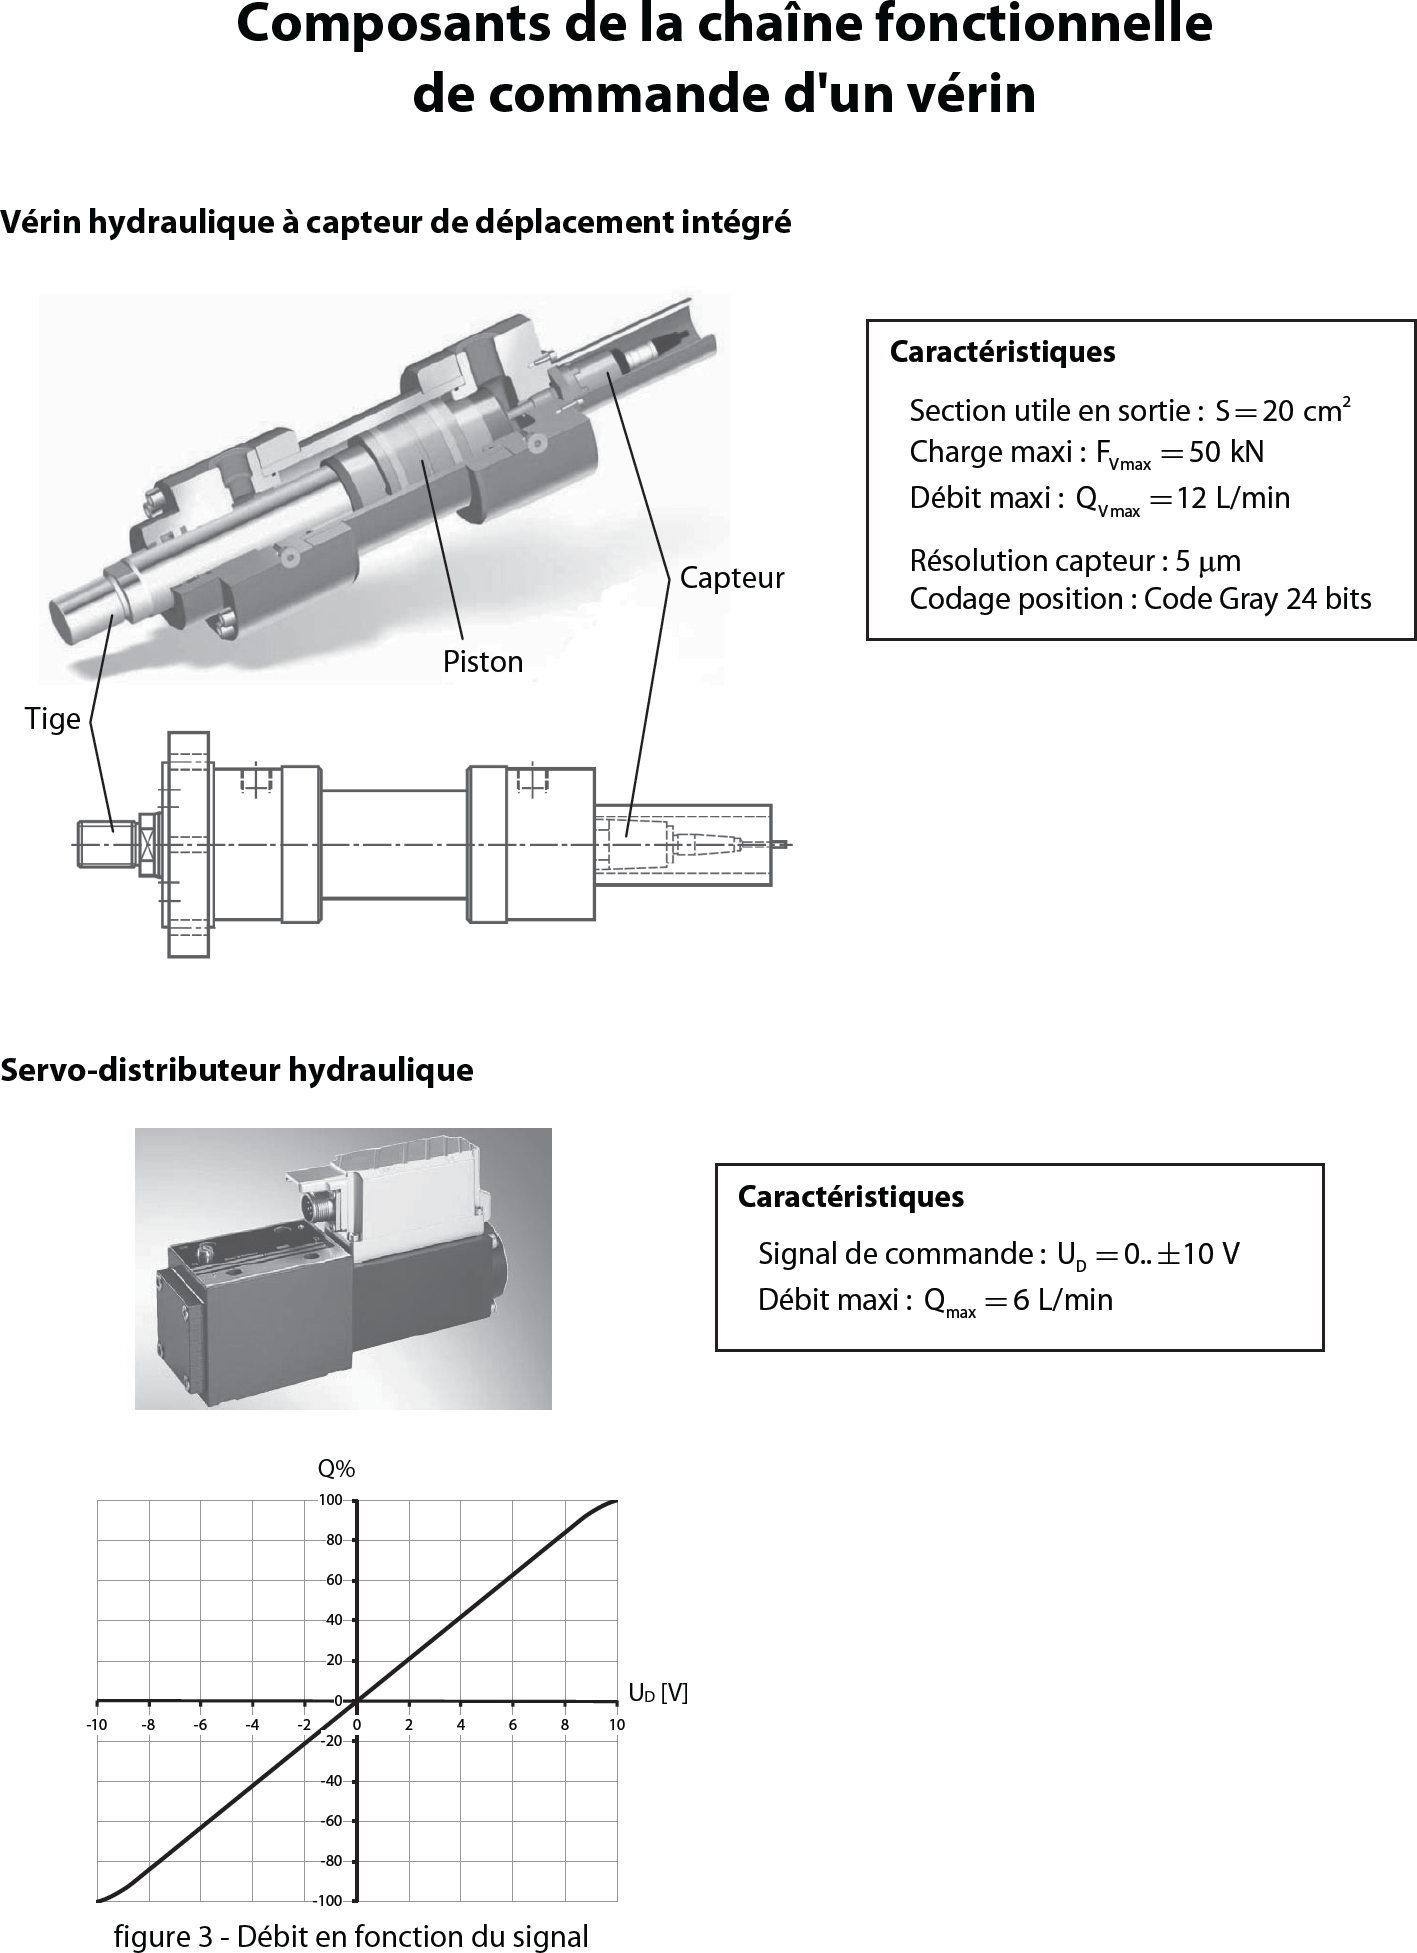
\includegraphics[width=\linewidth]{ann_b}
%\caption{\label{doc_05} Tuyère fermée}
\end{figure}

\subsection{\label{ann_03}Mécanisme de transmission de mouvement pour un volet}
\begin{figure}[H]
\centering
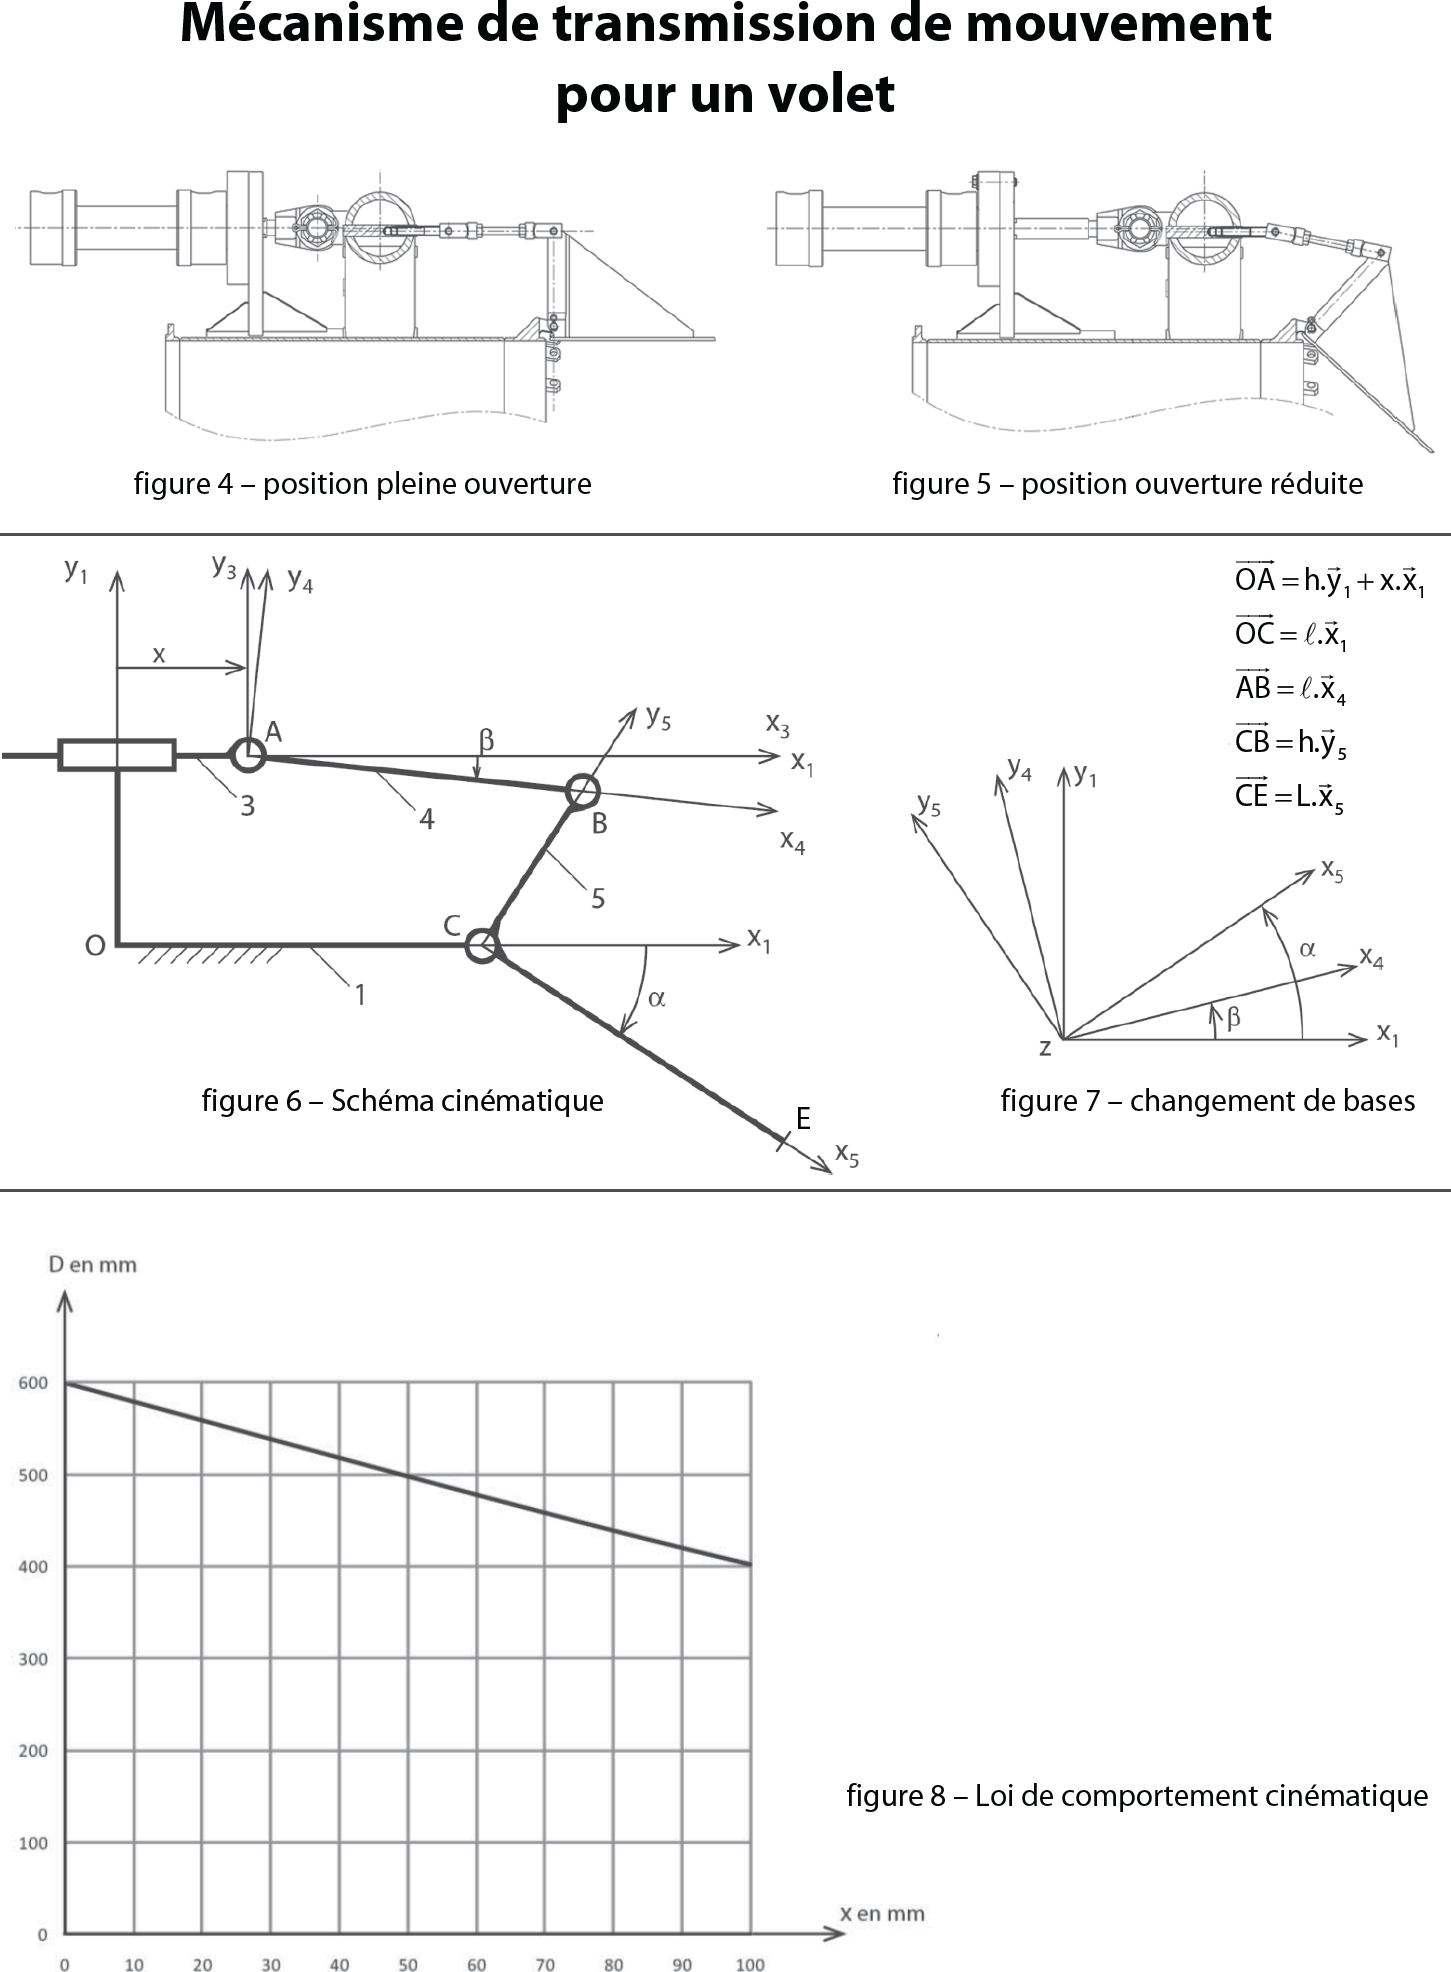
\includegraphics[width=\linewidth]{ann_c}
%\caption{\label{doc_05} Tuyère fermée}
\end{figure}

\subsection{\label{ann_04}Modélisation géométrique d'un volet}
\begin{figure}[H]
\centering
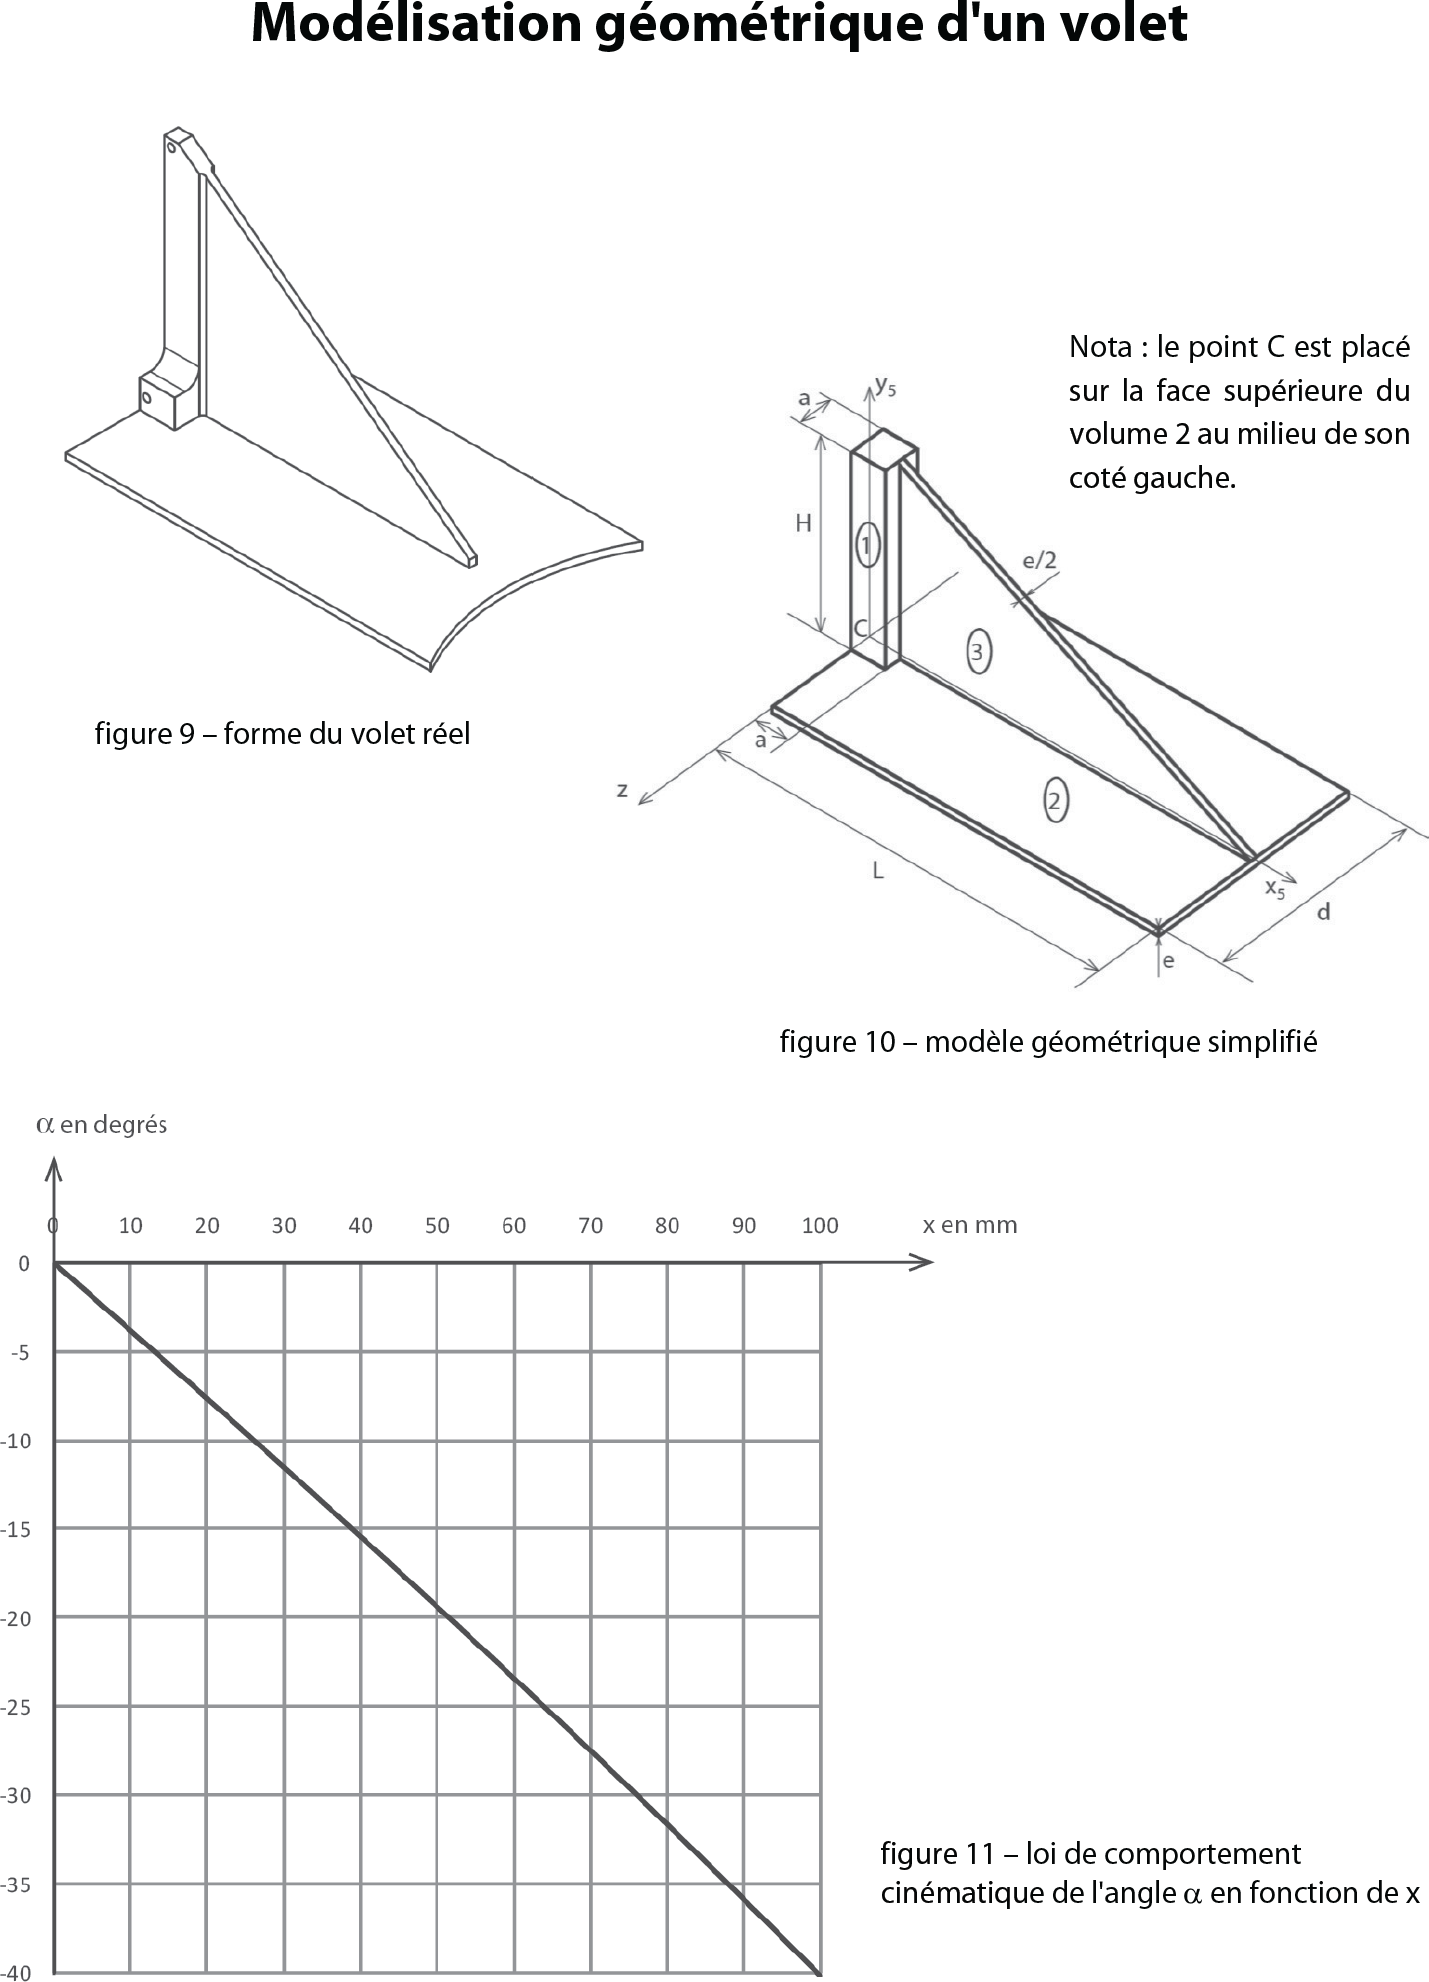
\includegraphics[width=\linewidth]{ann_d}
%\caption{\label{doc_05} Tuyère fermée}
\end{figure}

\newpage 
\section{Document réponse}


% Q33
\textbf{Question \ref{q_33}}

\begin{figure}[H]
\centering
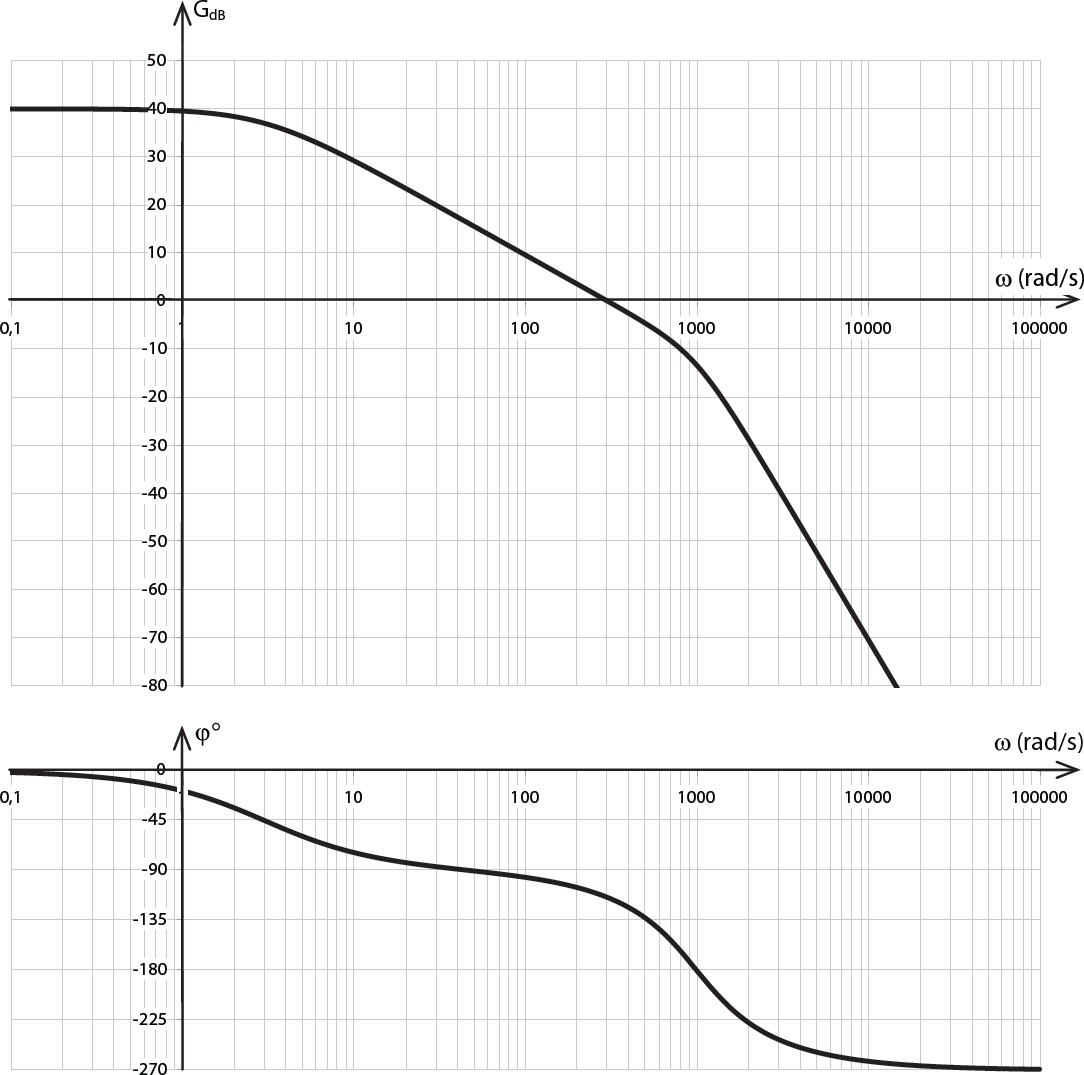
\includegraphics[width=\linewidth]{dr_Q33}
%\caption{\label{doc_05} Tuyère fermée}
\end{figure}
\end{document}

